
\phantomsection\label{am:The Garden Main Area Overview}
  \begin{landscape}
	\includepdf[angle=90, picturecommand*={}]{./maps/area/out/Garden_c.pdf}
  \end{landscape}


\thispagestyle{empty}
\colorlet{shadecolor}{\chapterColor}
\chapter{The Garden Main}

\fancyhead{}
\lhead[\textcolor{\chapterColor}{\rule[-2pt]{\textwidth}{15pt}}]{\textcolor{\chapterColor}{\rule[-2pt]{\textwidth}{15pt}}\hspace{-\textwidth}\color{white}\hspace{4pt}\protect\thepage\hspace{1ex}-\hspace{1ex}The Garden Main}
\rhead[\textcolor{\chapterColor}{\rule[-2pt]{\textwidth}{15pt}}\hspace{-\textwidth}\color{white}The Garden Main \protect\thepage \hspace{4pt}]{\textcolor{\chapterColor}{\rule[-2pt]{\textwidth}{15pt}}}
\fancyhead[RO]{}
\fancyhead[RE]{\color{white}The Garden Main\hspace{1ex}-\hspace{1ex}\protect\thepage \hspace{4pt}}


\raggedcolumns
\begin{multicols}{2}
\setbox0=\hbox{
\includegraphics[width=0.45\linewidth]{./maps/qr//The Garden Main_qr.png}}% Store image in \box0
\needspace{\ht0}% Need at least the height of \box0
\begin{center}

\includegraphics[width=0.45\linewidth]{./maps/qr//The Garden Main_qr.png}
\end{center}
\begin{center}
\underline{\textcolor{blue}{\href{http://maps.google.com/maps?q=44.44076010641458,-122.5752659013521}{Navigate to this area}}}
\end{center}


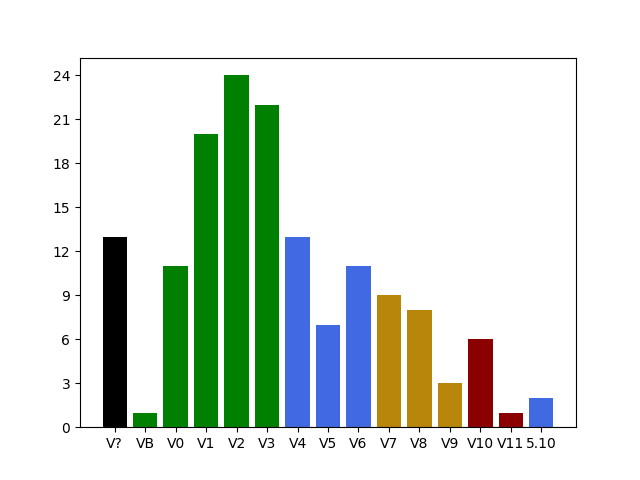
\includegraphics[width=\linewidth]{./maps/plots//The Garden Main.png}
\end{multicols}
\begin{multicols}{2}

Located about 3.5 miles down Quartzville Road from Highway 20, park in the gravel pull out where the road bends left just before you reach the boulders. The Garden Main bouldering area is true to its name. A lush green space features moss covered boulders situated under a dense canopy.\\



\null\newpage
\phantomsection\label{sm:Entrance Area map}
	\setbox0=\hbox{\begin{overpic}[width=0.8\linewidth]{./maps/area/out/entrance_c.png}
	\end{overpic}}
	\needspace{\ht0}
	\begin{center}
	\begin{overpic}[width=0.9\linewidth]{./maps/area/out/entrance_c.png}
	\end{overpic}
	\end{center}


\section{A - Entrance Area}\phantomsection\label{sa:Entrance Area}

A cluster of boulders situated in between the two main trails.\\



\phantomsection\label{tp:Toilet Bowl}
	\setbox0=\hbox{\begin{overpic}[width=0.8\linewidth]{./maps/topos/toilet_c.png}
	\end{overpic}}
	\needspace{\ht0}
	\begin{center}
	\begin{overpic}[width=0.9\linewidth]{./maps/topos/toilet_c.png}
	\end{overpic}
	\end{center}


\needspace{10em}
\subsection*{Toilet Bowl}\phantomsection\label{bf:Toilet Bowl}

If approaching via the main trail this is the first boulder you will encounter just off the road.\\



\needspace{2em}
\phantomsection\label{rt:Toilet Bowl}
\colorbox{green!20}{
\parbox{0.95\linewidth}{
\hspace{-1ex}\textbf{$\Box$
1 Toilet Bowl V1 \ding{72} 
}}}
\begin{adjustwidth}{1.3em}{}			

Stand start on a protruding block with left hand on an under cling and right hand on a knob. Pull a few moves to gain the lip of the boulder.
\end{adjustwidth}




\needspace{2em}
\phantomsection\label{rt:Toilet Bowl Traverse}
\colorbox{green!20}{
\parbox{0.95\linewidth}{
\hspace{-1ex}\textbf{$\Box$
2 Toilet Bowl Traverse V0 \ding{72}\ding{72} 
}}}
\begin{adjustwidth}{1.3em}{}			

Starting on a good rail at the lower left of the boulder. Traverse the lip topping out at the highest point or continue all the way until the boulder recedes into the hill.
\end{adjustwidth}



	\end{multicols}


	\begin{multicols}{2}

\phantomsection\label{tp:Overhand}
	\setbox0=\hbox{\begin{overpic}[width=0.8\linewidth]{./maps/topos/overhand2_c.png}
	\end{overpic}}
	\needspace{\ht0}
	\begin{center}
	\begin{overpic}[width=0.9\linewidth]{./maps/topos/overhand2_c.png}
	\end{overpic}
	\end{center}


\needspace{10em}
\subsection*{Overhand}\phantomsection\label{bf:Overhand}

a short prow in the rocky landscape between the two entrance trails.\\



\needspace{2em}
\phantomsection\label{rt:Overhand}
\colorbox{Goldenrod!20}{
\parbox{0.95\linewidth}{
\hspace{-1ex}\textbf{$\Box$
3 Overhand V8 \ding{72}\ding{72} \warn
}}}
\begin{adjustwidth}{1.3em}{}			

Climbs a short overhang starting at the bottom of the left arête. Try not to blow the last move. Also known as Evolve to Be More.
\end{adjustwidth}




	\end{multicols}
\phantomsection\label{tp:Boys in the Woods}
	\setbox0=\hbox{\begin{overpic}[width=0.8\linewidth]{./maps/topos/BITW_c.png}
	\end{overpic}}
	\needspace{\ht0}
	\begin{center}
	\begin{overpic}[width=0.9\linewidth]{./maps/topos/BITW_c.png}
	\end{overpic}
	\end{center}

	\begin{multicols}{2}

\needspace{10em}
\subsection*{Boys In the Woods}\phantomsection\label{bf:Boys In the Woods}

A low boulder with an identifiable scoop on the downhill side is located on the main trail roughly 150' uphill from the road.\\



\needspace{2em}
\phantomsection\label{rt:Boys in the Woods}
\colorbox{RoyalBlue!20}{
\parbox{0.95\linewidth}{
\hspace{-1ex}\textbf{$\Box$
4 Boys in the Woods V4 \ding{72}\ding{72} 
}}}
\begin{adjustwidth}{1.3em}{}			

Start on a low jug just before the scoop at the lowest part of the boulder. Climb up the left arête of the scoop until you can flop in. Some may consider this an eliminate since, with difficulty, you could also just mantle directly into the scoop.
\end{adjustwidth}


\begin{adjustwidth}{0.5cm}{}				
\needspace{4em}
\textbf{Variations:} \newline

\needspace{2em}
\phantomsection\label{vr:Tabor Tots}
\colorbox{black!20}{
\parbox{0.95\linewidth}{
\hspace{-1ex}\textbf{$\Box$
4a Tabor Tots V?  
}}}
\begin{adjustwidth}{1.3em}{}			

Climb boys in the woods, but instead of topping traverse left along the lip of the boulder all the way to the apex on the back side. Also called "A Boy and His Wood". Unclear if this has actually been done before.
\end{adjustwidth}



\end{adjustwidth}


\needspace{2em}
\phantomsection\label{rt:Cuba Gooding}
\colorbox{RoyalBlue!20}{
\parbox{0.95\linewidth}{
\hspace{-1ex}\textbf{$\Box$
5 Cuba Gooding V6 \ding{72}\ding{72} 
}}}
\begin{adjustwidth}{1.3em}{}			

Start as for Boys in the Woods but climb right along the lip of the scoop into the top of Ice Cubes Shiny Jerry Curl. Contrived.
\end{adjustwidth}


\begin{adjustwidth}{0.5cm}{}				
\needspace{4em}
\textbf{Variations:} \newline

\needspace{2em}
\phantomsection\label{vr:EZe}
\colorbox{green!20}{
\parbox{0.95\linewidth}{
\hspace{-1ex}\textbf{$\Box$
5a EZe V3 \ding{72} 
}}}
\begin{adjustwidth}{1.3em}{}			

Climb Cuba Gooding but use good holds to pull into the scoop and exit early.
\end{adjustwidth}



\end{adjustwidth}


\needspace{2em}
\phantomsection\label{rt:Ice Cubes Shiny Jerry Curl}
\colorbox{RoyalBlue!20}{
\parbox{0.95\linewidth}{
\hspace{-1ex}\textbf{$\Box$
6 Ice Cubes Shiny Jerry Curl V6 \ding{72}\ding{72} 
}}}
\begin{adjustwidth}{1.3em}{}			

Sit start on a low sloping edge and make a huge reach to gain sharp crimps in thin horizontal seams at eye level.
\end{adjustwidth}



\phantomsection\label{tp:Spider Bumps}
	\setbox0=\hbox{\begin{overpic}[width=0.8\linewidth]{./maps/topos/spiderBumps_c.png}
	\end{overpic}}
	\needspace{\ht0}
	\begin{center}
	\begin{overpic}[width=0.9\linewidth]{./maps/topos/spiderBumps_c.png}
	\end{overpic}
	\end{center}


\needspace{2em}
\phantomsection\label{rt:Spider Bumps}
\colorbox{RoyalBlue!20}{
\parbox{0.95\linewidth}{
\hspace{-1ex}\textbf{$\Box$
7 Spider Bumps V4 \ding{72} 
}}}
\begin{adjustwidth}{1.3em}{}			

Start on a thin crimp rail over a dabby rock. Maneuver yourself to a good jug using almost non existent holds while trying not to dab.
\end{adjustwidth}





\needspace{10em}
\subsection*{Tree Slab}\phantomsection\label{bf:Tree Slab}

A narrow slab just uphill and to the right of the Boys in the Woods boulder.\\



\needspace{2em}
\phantomsection\label{rt:Tree Slab}
\colorbox{green!20}{
\parbox{0.95\linewidth}{
\hspace{-1ex}\textbf{$\Box$
8 Tree Slab V1+ \ding{72}\ding{72} 
}}}
\begin{adjustwidth}{1.3em}{}			

Climb the center of the slab from a stand start.
\end{adjustwidth}




\phantomsection\label{tp:The Good Warm Up}
	\setbox0=\hbox{\begin{overpic}[width=0.8\linewidth]{./maps/topos/goodWarmUp_c.png}
	\end{overpic}}
	\needspace{\ht0}
	\begin{center}
	\begin{overpic}[width=0.9\linewidth]{./maps/topos/goodWarmUp_c.png}
	\end{overpic}
	\end{center}


\needspace{10em}
\subsection*{The Good Warm Up}\phantomsection\label{bf:The Good Warm Up}

A tiny fin shaped boulder on the main trail.\\



\needspace{2em}
\phantomsection\label{rt:The Good Warm Up}
\colorbox{green!20}{
\parbox{0.95\linewidth}{
\hspace{-1ex}\textbf{$\Box$
9 The Good Warm Up V0 \ding{72} 
}}}
\begin{adjustwidth}{1.3em}{}			

Whether or not this is a good warmup is debatable. Sit start with hands matched on a good rail. Climb the short face using both arêtes. Also known as Shark Fin.
\end{adjustwidth}





\needspace{10em}
\subsection*{Tonsil}\phantomsection\label{bf:Tonsil}

A small hanging prow wedged under a larger hanging prow, which is itself wedged under the Meth Lab prow (a very big hanging prow).\\


\phantomsection\label{tp:Tonsil}
	\setbox0=\hbox{\begin{overpic}[width=0.8\linewidth]{./maps/topos/tonsil2_c.png}
	\end{overpic}}
	\needspace{\ht0}
	\begin{center}
	\begin{overpic}[width=0.9\linewidth]{./maps/topos/tonsil2_c.png}
	\end{overpic}
	\end{center}


\needspace{2em}
\phantomsection\label{rt:Tonsil}
\colorbox{RoyalBlue!20}{
\parbox{0.95\linewidth}{
\hspace{-1ex}\textbf{$\Box$
10 Tonsil V4 \ding{72}\ding{72} 
}}}
\begin{adjustwidth}{1.3em}{}			

Step off the boulder below to gain high starting holds. Begin in compression with right hand on a vertical side pull sloper on the blunt right corner and left hand on a juggy under cling.  Shorter climbers will have difficulty reaching the starting holds. After establishing the rock below is off.
\end{adjustwidth}


\begin{adjustwidth}{0.5cm}{}				
\needspace{4em}
\textbf{Variations:} \newline

\needspace{2em}
\phantomsection\label{vr:Tonsil Low Start}
\colorbox{black!20}{
\parbox{0.95\linewidth}{
\hspace{-1ex}\textbf{$\Box$
10a Tonsil Low Start V?  
}}}
\begin{adjustwidth}{1.3em}{}			

Climb tonsil from the obvious lower holds without using the boulder below it as a foot. Rumor has it that this has been done.
  (No Topo)
\end{adjustwidth}




\needspace{2em}
\phantomsection\label{vr:Prowed}
\colorbox{black!20}{
\parbox{0.95\linewidth}{
\hspace{-1ex}\textbf{$\Box$
10b Prowed V?  \warn\warn
}}}
\begin{adjustwidth}{1.3em}{}			

Climb tonsil but instead of doing the normal top out, continue climbing the steep prow above it. Reportedly this was an old school classic.
\end{adjustwidth}



\end{adjustwidth}


\needspace{2em}
\phantomsection\label{rt:Gingiva}
\colorbox{green!20}{
\parbox{0.95\linewidth}{
\hspace{-1ex}\textbf{$\Box$
11 Gingiva* V2 \ding{72} 
}}}
\begin{adjustwidth}{1.3em}{}			

Climbs the boulder below Tonsil. Sit start with low holds on the right arête. Pull a few awkward moves into a cramped top out.
\end{adjustwidth}




\phantomsection\label{tp:All Sorts of Ease}
	\setbox0=\hbox{\begin{overpic}[width=0.8\linewidth]{./maps/topos/ease_c.png}
	\end{overpic}}
	\needspace{\ht0}
	\begin{center}
	\begin{overpic}[width=0.9\linewidth]{./maps/topos/ease_c.png}
	\end{overpic}
	\end{center}


\needspace{10em}
\subsection*{All Sorts of Ease}\phantomsection\label{bf:All Sorts of Ease}

A low angle slab under the Meth Lab prow.\\



\needspace{2em}
\phantomsection\label{rt:All Sorts of Ease}
\colorbox{green!20}{
\parbox{0.95\linewidth}{
\hspace{-1ex}\textbf{$\Box$
12 All Sorts of Ease VB \ding{72}\ding{72} 
}}}
\begin{adjustwidth}{1.3em}{}			

Climb the left side of the face on good holds. Fun.
\end{adjustwidth}




\needspace{2em}
\phantomsection\label{rt:In the Shadow of Giants}
\colorbox{green!20}{
\parbox{0.95\linewidth}{
\hspace{-1ex}\textbf{$\Box$
13 In the Shadow of Giants V2 \ding{72} 
}}}
\begin{adjustwidth}{1.3em}{}			

Stand start with wide hands. Left hand on thin pinch at head height and right hang on a slightly higher small lumpy edge with a thumb catch. Pull a few delicate moves to gain the lip. A sit start looks doable, but unpleasant.
\end{adjustwidth}




\phantomsection\label{tp:Three Star Ledge}
	\setbox0=\hbox{\begin{overpic}[width=0.8\linewidth]{./maps/topos/threeStar2_c.png}
	\end{overpic}}
	\needspace{\ht0}
	\begin{center}
	\begin{overpic}[width=0.9\linewidth]{./maps/topos/threeStar2_c.png}
	\end{overpic}
	\end{center}


\needspace{10em}
\subsection*{Three Star Ledge}\phantomsection\label{bf:Three Star Ledge}

Angular boulder in the rocky landscape between the two entrance trails.\\



\needspace{2em}
\phantomsection\label{rt:Three Star Ledge}
\colorbox{green!20}{
\parbox{0.95\linewidth}{
\hspace{-1ex}\textbf{$\Box$
14 Three Star Ledge V2 \ding{72}\ding{72} 
}}}
\begin{adjustwidth}{1.3em}{}			

Stand start with hands matched on the ledge. Chuck out to the left arête and follow it to the apex of the boulder. The small boulders at the base are off.
\end{adjustwidth}


\begin{adjustwidth}{0.5cm}{}				
\needspace{4em}
\textbf{Variations:} \newline

\needspace{2em}
\phantomsection\label{vr:Three Star Ledge Variation}
\colorbox{green!20}{
\parbox{0.95\linewidth}{
\hspace{-1ex}\textbf{$\Box$
14a Three Star Ledge Variation V2 \ding{72}\ding{72} 
}}}
\begin{adjustwidth}{1.3em}{}			

Squat start with feet on the small boulder below 3 star (it's on this time!) and hands on opposing under clings.
\end{adjustwidth}



\end{adjustwidth}


\phantomsection\label{tp:Turtle}
	\setbox0=\hbox{\begin{overpic}[width=0.8\linewidth]{./maps/topos/turtle_c.png}
	\end{overpic}}
	\needspace{\ht0}
	\begin{center}
	\begin{overpic}[width=0.9\linewidth]{./maps/topos/turtle_c.png}
	\end{overpic}
	\end{center}


\needspace{10em}
\subsection*{Turtle Shell Boulder}\phantomsection\label{bf:Turtle Shell Boulder}

A short boulder with a low angle off-width crack. If approaching on the fight club trail this is the first boulder that you will encounter\\



\needspace{2em}
\phantomsection\label{rt:Raphael Crack}
\colorbox{green!20}{
\parbox{0.95\linewidth}{
\hspace{-1ex}\textbf{$\Box$
15 Raphael Crack V0 \ding{72} 
}}}
\begin{adjustwidth}{1.3em}{}			

Climb the wide crack from a stand start.
\end{adjustwidth}




\needspace{2em}
\phantomsection\label{rt:Donatello}
\colorbox{green!20}{
\parbox{0.95\linewidth}{
\hspace{-1ex}\textbf{$\Box$
16 Donatello V1 \ding{72} 
}}}
\begin{adjustwidth}{1.3em}{}			

start on a flat ledge where the rock angle changes. Slap a low angle arête until you can hike your feet up. Only somewhat distinct from Leonardo.
\end{adjustwidth}




\needspace{2em}
\phantomsection\label{rt:Leonardo}
\colorbox{green!20}{
\parbox{0.95\linewidth}{
\hspace{-1ex}\textbf{$\Box$
17 Leonardo V3 \ding{72} 
}}}
\begin{adjustwidth}{1.3em}{}			

Lay down start with hands on a low broken flake. With difficulty pull off the ground and slap a slopey ledge traverse up and left until you can rock over onto the downhill face. Sort of like a worse version of boys in the woods.
\end{adjustwidth}


\begin{adjustwidth}{0.5cm}{}				
\needspace{4em}
\textbf{Variations:} \newline

\needspace{2em}
\phantomsection\label{vr:Turtle Traverse}
\colorbox{RoyalBlue!20}{
\parbox{0.95\linewidth}{
\hspace{-1ex}\textbf{$\Box$
17a Turtle Traverse V4 \ding{72}\ding{72} 
}}}
\begin{adjustwidth}{1.3em}{}			

Start as for Leonardo, but stay low and traverse left into Raphael Crack. Not quite as contrived as it looks.
\end{adjustwidth}



\end{adjustwidth}



\null\newpage
	\end{multicols}
\phantomsection\label{sm:Fight Club Area map}
	\setbox0=\hbox{\begin{overpic}[width=0.8\linewidth]{./maps/area/out/fightClub_c.png}
	\end{overpic}}
	\needspace{\ht0}
	\begin{center}
	\begin{overpic}[width=0.9\linewidth]{./maps/area/out/fightClub_c.png}
	\end{overpic}
	\end{center}

	\begin{multicols}{2}

\section{B - Fight Club}\phantomsection\label{sa:Fight Club}

Located in the southwest corner of the Garden main, the Fight Club zone is home to the namesake V8 test piece as well as several other quality lines. Flat landings and easy access make this a nice spot to spend some time\\




\needspace{10em}
\subsection*{The Office}\phantomsection\label{bf:The Office}

A tall not quite vertical boulder is immediately on your right as you enter the Fight Club area.\\



\needspace{2em}
\phantomsection\label{rt:Dwight Schrute}
\colorbox{green!20}{
\parbox{0.95\linewidth}{
\hspace{-1ex}\textbf{$\Box$
1 Dwight Schrute V1 \ding{72}\ding{72} \warn
}}}
\begin{adjustwidth}{1.3em}{}			

Climb the slab over a narrow, but flat landing.
\end{adjustwidth}




\needspace{2em}
\phantomsection\label{rt:Jim Halpert}
\colorbox{green!20}{
\parbox{0.95\linewidth}{
\hspace{-1ex}\textbf{$\Box$
2 Jim Halpert V1* \ding{73} \warn\warn
}}}
\begin{adjustwidth}{1.3em}{}			

Starting on the right edge of the block climb climb the right corner over a rocky landing. Either pull some harder moves to stay on the downhill face or round the corner to the right and pull some easier moves over a worse landing. Grade and rating unconfirmed.
\end{adjustwidth}




\needspace{2em}
\phantomsection\label{rt:Michael Scott}
\colorbox{green!20}{
\parbox{0.95\linewidth}{
\hspace{-1ex}\textbf{$\Box$
3 Michael Scott V3 \ding{72}\ding{72} \warn
}}}
\begin{adjustwidth}{1.3em}{}			

Climb the center of the boulder using a cool sloper and some perchy feet.
\end{adjustwidth}




\needspace{2em}
\phantomsection\label{rt:Daryl Philbin}
\colorbox{green!20}{
\parbox{0.95\linewidth}{
\hspace{-1ex}\textbf{$\Box$
4 Daryl Philbin V1/2 \ding{72}\ding{72}\ding{72} \warn
}}}
\begin{adjustwidth}{1.3em}{}			

Starting at the Center of the block climb left on good holds to the arête. Climb up the arête until you can reach good face holds up right and continue through a, thankfully, juggy top out. Left and right alternative starts add a little variety but do not change the grade. Mind the rock at the base of the climb. This line was originally referred to as The Burning Bus in reference to an unfortunate hitch hiker that was encountered on the road in.
\end{adjustwidth}




\needspace{2em}
\phantomsection\label{rt:Backside of Office}
\colorbox{black!20}{
\parbox{0.95\linewidth}{
\hspace{-1ex}\textbf{$\Box$
5 Routes on the Backside V?  
}}}
\begin{adjustwidth}{1.3em}{}			

The faces on the backside of this boulder have been discovered and forgotten several times over the years. Reestablishing these lines is a project for the future.
  (No Topo)
\end{adjustwidth}




	\end{multicols}
\phantomsection\label{tp:Office}
	\setbox0=\hbox{\begin{overpic}[width=0.8\linewidth]{./maps/topos/office_c.png}
	\end{overpic}}
	\needspace{\ht0}
	\begin{center}
	\begin{overpic}[width=0.9\linewidth]{./maps/topos/office_c.png}
	\end{overpic}
	\end{center}

	\begin{multicols}{2}

\needspace{10em}
\subsection*{Crash Test Dummies}\phantomsection\label{bf:Crash Test Dummies}

A small boulder in between The Office and Fight Club.\\



\needspace{2em}
\phantomsection\label{rt:Vince}
\colorbox{green!20}{
\parbox{0.95\linewidth}{
\hspace{-1ex}\textbf{$\Box$
6 Vince V2 \ding{72}\ding{72} 
}}}
\begin{adjustwidth}{1.3em}{}			

Squat start on good edges. Navigate a crescent shaped side pull rail to a delicate top out. Make sure to clean the top out before attempting.
\end{adjustwidth}




\phantomsection\label{tp:Fight Club Right Side}
	\setbox0=\hbox{\begin{overpic}[width=0.8\linewidth]{./maps/topos/fightClub_c.png}
	\end{overpic}}
	\needspace{\ht0}
	\begin{center}
	\begin{overpic}[width=0.9\linewidth]{./maps/topos/fightClub_c.png}
	\end{overpic}
	\end{center}


\needspace{10em}
\subsection*{Fight Club}\phantomsection\label{bf:Fight Club}

The obvious overhanging boulder with an interesting bubbly texture.\\



\needspace{2em}
\phantomsection\label{rt:The Ear}
\colorbox{green!20}{
\parbox{0.95\linewidth}{
\hspace{-1ex}\textbf{$\Box$
7 The Ear V3 \ding{72}\ding{72}\ding{72} 
}}}
\begin{adjustwidth}{1.3em}{}			

Start on the arête at the far right end of the boulder. Climb straight up through tricky holds to a heady top out. Veering onto the face instead of using the good holds on the right arête bumps the grade up to around V4.
\end{adjustwidth}




\needspace{2em}
\phantomsection\label{rt:Fight Club}
\colorbox{Goldenrod!20}{
\parbox{0.95\linewidth}{
\hspace{-1ex}\textbf{$\Box$
8 Fight Club V8 \ding{72}\ding{72}\ding{72} 
}}}
\begin{adjustwidth}{1.3em}{}			

Area classic, this rig is a feather in any would be crushers cap. Start on the far right arête as for Ear. Traverse across the angle change and top out above a bubbly crimp rail on the overhanging face.
\end{adjustwidth}



\phantomsection\label{tp:Fight Club Left Side}
	\setbox0=\hbox{\begin{overpic}[width=0.8\linewidth]{./maps/topos/fightClub2_c.png}
	\end{overpic}}
	\needspace{\ht0}
	\begin{center}
	\begin{overpic}[width=0.9\linewidth]{./maps/topos/fightClub2_c.png}
	\end{overpic}
	\end{center}


\needspace{2em}
\phantomsection\label{rt:Fight Club 2}
\colorbox{red!20}{
\parbox{0.95\linewidth}{
\hspace{-1ex}\textbf{$\Box$
9 Fight Club 2 V10 \ding{72}\ding{72} 
}}}
\begin{adjustwidth}{1.3em}{}			

Sit start with hands matched low on the left arête of the overhanging boulder. Climb across the overhang topping as for Fight Club.
\end{adjustwidth}




\needspace{2em}
\phantomsection\label{rt:Brewmaster}
\colorbox{RoyalBlue!20}{
\parbox{0.95\linewidth}{
\hspace{-1ex}\textbf{$\Box$
10 Brewmaster V5 \ding{72}\ding{72} 
}}}
\begin{adjustwidth}{1.3em}{}			

Not to be mistaken for Fight Club 2. Sit start in the same spot but climb up the arête. Starting a move or two in brings the grade down a bit. This is also known as tool shed direct.
\end{adjustwidth}




\phantomsection\label{tp:Trust}
	\setbox0=\hbox{\begin{overpic}[width=0.8\linewidth]{./maps/topos/trust_c.png}
	\end{overpic}}
	\needspace{\ht0}
	\begin{center}
	\begin{overpic}[width=0.9\linewidth]{./maps/topos/trust_c.png}
	\end{overpic}
	\end{center}


\needspace{10em}
\subsection*{Tyler Durten}\phantomsection\label{bf:Tyler Durten}

Just to the left of the fight club boulder is a tall wall with few features other than a distinctive crimp rail at eye level.\\



\needspace{2em}
\phantomsection\label{rt:Project Mayhem}
\colorbox{green!20}{
\parbox{0.95\linewidth}{
\hspace{-1ex}\textbf{$\Box$
11 Project Mayhem V1+ \ding{72} 
}}}
\begin{adjustwidth}{1.3em}{}			

Start on a heinous crimp rail and punch out left to much better holds.
\end{adjustwidth}


\begin{adjustwidth}{0.5cm}{}				
\needspace{4em}
\textbf{Variations:} \newline

\needspace{2em}
\phantomsection\label{vr:Tyler Durten Dyno}
\colorbox{black!20}{
\parbox{0.95\linewidth}{
\hspace{-1ex}\textbf{$\Box$
11a Tyler Durten Dyno V?  
}}}
\begin{adjustwidth}{1.3em}{}			

It has been speculated that the dyno from the starting hold straight to the lip will go.
\end{adjustwidth}



\end{adjustwidth}


\needspace{2em}
\phantomsection\label{rt:Angel Face}
\colorbox{RoyalBlue!20}{
\parbox{0.95\linewidth}{
\hspace{-1ex}\textbf{$\Box$
12 Angel Face V6*  
}}}
\begin{adjustwidth}{1.3em}{}			

Start as for Tyler Durten but climb more or less straight up using the sloping rib on the upper right side of the boulder
\end{adjustwidth}




\needspace{2em}
\phantomsection\label{rt:Durten Layback}
\colorbox{green!20}{
\parbox{0.95\linewidth}{
\hspace{-1ex}\textbf{$\Box$
13 Durten Layback V1 \ding{72} 
}}}
\begin{adjustwidth}{1.3em}{}			

Stand start and climb the right corner using the Fight Club boulder for feet. Is chimneying between the boulders off? Asking for a friend.
\end{adjustwidth}





\needspace{10em}
\subsection*{Trust}\phantomsection\label{bf:Trust}

The Trust boulder sits on an terrace behind Mini Me and to the Left of Tyler Durten.\\



\needspace{2em}
\phantomsection\label{rt:Trust}
\colorbox{green!20}{
\parbox{0.95\linewidth}{
\hspace{-1ex}\textbf{$\Box$
14 Trust V2 \ding{72}\ding{72}\ding{72} 
}}}
\begin{adjustwidth}{1.3em}{}			

Sit start in compression on a hanging refrigerator block. Climb straight up through a sloping ledge to the top. Look for the juggy crack ~1ft inset from the lip.
\end{adjustwidth}


\begin{adjustwidth}{0.5cm}{}				
\needspace{4em}
\textbf{Variations:} \newline

\needspace{2em}
\phantomsection\label{vr:Iron Cross}
\colorbox{green!20}{
\parbox{0.95\linewidth}{
\hspace{-1ex}\textbf{$\Box$
14a Iron Cross V2 \ding{72} 
}}}
\begin{adjustwidth}{1.3em}{}			

Avoid the committing moves at the lip by traversing left early.
\end{adjustwidth}



\end{adjustwidth}


\phantomsection\label{tp:Mini Me}
	\setbox0=\hbox{\begin{overpic}[width=0.8\linewidth]{./maps/topos/miniMe_c.png}
	\end{overpic}}
	\needspace{\ht0}
	\begin{center}
	\begin{overpic}[width=0.9\linewidth]{./maps/topos/miniMe_c.png}
	\end{overpic}
	\end{center}


\needspace{10em}
\subsection*{Mini Me}\phantomsection\label{bf:Mini Me}

A short pointy boulder with a flat landing is nearly freestanding on the downhill side of the Fight Club zone.\\



\needspace{2em}
\phantomsection\label{rt:Mini Me}
\colorbox{green!20}{
\parbox{0.95\linewidth}{
\hspace{-1ex}\textbf{$\Box$
15 Mini Me V3 \ding{72} 
}}}
\begin{adjustwidth}{1.3em}{}			

start on blunt corner. Make tricky moves to a blocky jug to the lip and traverse left to an easy top over a rocky landing.
\end{adjustwidth}




\needspace{2em}
\phantomsection\label{rt:Austin Powers}
\colorbox{RoyalBlue!20}{
\parbox{0.95\linewidth}{
\hspace{-1ex}\textbf{$\Box$
16 Austin Powers V5 \ding{72}\ding{72} 
}}}
\begin{adjustwidth}{1.3em}{}			

Start straddling a blunt corner with your left hand on a lemon sized knob and right on a low side pull crimp, Crank to a jug and move right into top of Dr. Evil. Also known as Macro Me. Starting as for Mini Me is also a valid interpretation of this line.
\end{adjustwidth}



\phantomsection\label{tp:Mini Me 2}
	\setbox0=\hbox{\begin{overpic}[width=0.8\linewidth]{./maps/topos/drEvil_c.png}
	\end{overpic}}
	\needspace{\ht0}
	\begin{center}
	\begin{overpic}[width=0.9\linewidth]{./maps/topos/drEvil_c.png}
	\end{overpic}
	\end{center}


\needspace{2em}
\phantomsection\label{rt:Dr. Evil}
\colorbox{RoyalBlue!20}{
\parbox{0.95\linewidth}{
\hspace{-1ex}\textbf{$\Box$
17 Dr. Evil V4 \ding{72}\ding{72} 
}}}
\begin{adjustwidth}{1.3em}{}			

sit start in compression with left hand on a low sloper side pull and right hand on the arête. Pull some tricky moves to gain better holds either rolling onto the right hand slab early or staying on the arête the whole way. Starting "one move in" with your right hand on the good obvious side pull is an all together more enjoyable experience if a little easier.
\end{adjustwidth}


\begin{adjustwidth}{0.5cm}{}				
\needspace{4em}
\textbf{Variations:} \newline

\needspace{2em}
\phantomsection\label{vr:Mr. Bigglesworth}
\colorbox{green!20}{
\parbox{0.95\linewidth}{
\hspace{-1ex}\textbf{$\Box$
17a Mr. Bigglesworth V1 \ding{72}\ding{72} 
}}}
\begin{adjustwidth}{1.3em}{}			

Start on your choice of waist high holds, climb straight up the right face or stay left on the arête. Authors note: other guides identify several other variations on this route, this book intentionally omits other variations in preference of encouraging climbers to find their own beta.
\end{adjustwidth}



\end{adjustwidth}


\phantomsection\label{tp:E's Dirty B}
	\setbox0=\hbox{\begin{overpic}[width=0.8\linewidth]{./maps/topos/eDirty_c.png}
	\end{overpic}}
	\needspace{\ht0}
	\begin{center}
	\begin{overpic}[width=0.9\linewidth]{./maps/topos/eDirty_c.png}
	\end{overpic}
	\end{center}


\needspace{10em}
\subsection*{E's Dirty B}\phantomsection\label{bf:E's Dirty B}

Following a faint trail west traveling past the trust boulder brings you to a Large boulder which almost immediately gives way to low angle slab.\\



\needspace{2em}
\phantomsection\label{rt:Green Hell}
\colorbox{green!20}{
\parbox{0.95\linewidth}{
\hspace{-1ex}\textbf{$\Box$
18 Green Hell V2 \ding{72}\ding{72} 
}}}
\begin{adjustwidth}{1.3em}{}			

Squat start on an angled rail at chest level to the left of the cave. The path of least resistance leads left but climbing straight up is also possible at a similar grade.
\end{adjustwidth}




\needspace{2em}
\phantomsection\label{rt:E's Dirty B}
\colorbox{RoyalBlue!20}{
\parbox{0.95\linewidth}{
\hspace{-1ex}\textbf{$\Box$
19 E's Dirty B V5 \ding{72}\ding{72} 
}}}
\begin{adjustwidth}{1.3em}{}			

Start with hands matched on a lumpy flake in the back of a small cave. Using sloping edges out right and a difficult under cling navigate out of the cave trending right at the lip to a jug. The final slab quest is an enjoyable and easy top out. Also known as Trouble with Bubbles.
\end{adjustwidth}




\needspace{2em}
\phantomsection\label{rt:Unknown on E's Dirty B}
\colorbox{green!20}{
\parbox{0.95\linewidth}{
\hspace{-1ex}\textbf{$\Box$
20 Unknown V1/2 \ding{72} 
}}}
\begin{adjustwidth}{1.3em}{}			

A hard squat start on a faint ripple leads to easier climbing. Starts just right of the cave.
\end{adjustwidth}






	\end{multicols}


	\begin{multicols}{2}

\null\newpage
\phantomsection\label{sm:Undertow area map}
	\setbox0=\hbox{\begin{overpic}[width=0.8\linewidth]{./maps/area/out/undertow_c.png}
	\end{overpic}}
	\needspace{\ht0}
	\begin{center}
	\begin{overpic}[width=0.9\linewidth]{./maps/area/out/undertow_c.png}
	\end{overpic}
	\end{center}


\section{C - Undertow}\phantomsection\label{sa:Undertow}

Directly uphill from Fight Club are a few quality boulders separated by overgrown trails.\\




\needspace{10em}
\subsection*{Silly Steep}\phantomsection\label{bf:Silly Steep}

Thin overhanging block left of the Undertow boulder.\\



\needspace{2em}
\phantomsection\label{rt:Silly Steep Mantle}
\colorbox{RoyalBlue!20}{
\parbox{0.95\linewidth}{
\hspace{-1ex}\textbf{$\Box$
1 Silly Steep Mantle V4 \ding{72}\ding{72} 
}}}
\begin{adjustwidth}{1.3em}{}			

Stand start with good compression holds in the roof. Make a hard pull to the juggy edge below the lip and figure out how to get your body over the top. Starting from the juggy edge knocks the grade down to V2/3. This route is also known as Flipside.
\end{adjustwidth}




	\end{multicols}
\phantomsection\label{tp:Undertow2}
	\setbox0=\hbox{\begin{overpic}[width=0.8\linewidth]{./maps/topos/undertow2_c.png}
	\end{overpic}}
	\needspace{\ht0}
	\begin{center}
	\begin{overpic}[width=0.9\linewidth]{./maps/topos/undertow2_c.png}
	\end{overpic}
	\end{center}

	\begin{multicols}{2}



\needspace{10em}
\subsection*{Undertow}\phantomsection\label{bf:Undertow}

Relatively off the beaten path as far as classic garden boulders goes. Follow a faint trail up hill past the trust boulder.\\



\needspace{2em}
\phantomsection\label{rt:Spray Skirt}
\colorbox{Goldenrod!20}{
\parbox{0.95\linewidth}{
\hspace{-1ex}\textbf{$\Box$
2 Spray Skirt V8 \ding{72}\ding{72} 
}}}
\begin{adjustwidth}{1.3em}{}			

Sit start with left hand in a slopey dish and right hand on a low side pull. Pull some bizarre moves to gain the "boob holds" at the start of Undertow, continue up and left through a series of heinous crimps. Avoid standing on Silly Steep and Mantle.
\end{adjustwidth}



\phantomsection\label{tp:Undertow}
	\setbox0=\hbox{\begin{overpic}[width=0.8\linewidth]{./maps/topos/undertow_c.png}
	\end{overpic}}
	\needspace{\ht0}
	\begin{center}
	\begin{overpic}[width=0.9\linewidth]{./maps/topos/undertow_c.png}
	\end{overpic}
	\end{center}


\needspace{2em}
\phantomsection\label{rt:Undertow}
\colorbox{green!20}{
\parbox{0.95\linewidth}{
\hspace{-1ex}\textbf{$\Box$
3 Undertow V3 \ding{72}\ding{72}\ding{72} 
}}}
\begin{adjustwidth}{1.3em}{}			

Start on two boob shaped slopers at head height. Climb straight up using face holds and the right arête.
\end{adjustwidth}


\begin{adjustwidth}{0.5cm}{}				
\needspace{4em}
\textbf{Variations:} \newline

\needspace{2em}
\phantomsection\label{vr:Spray Against the Undertow}
\colorbox{RoyalBlue!20}{
\parbox{0.95\linewidth}{
\hspace{-1ex}\textbf{$\Box$
3a Spray Against the Undertow V6 \ding{72}\ding{72} 
}}}
\begin{adjustwidth}{1.3em}{}			

Sit start as for Spray Skirt, climb into Undertow. This route is also called Dark Crystal.
\end{adjustwidth}




\needspace{2em}
\phantomsection\label{vr:Undertow Sit Start}
\colorbox{Goldenrod!20}{
\parbox{0.95\linewidth}{
\hspace{-1ex}\textbf{$\Box$
3b Undertow Sit Start V7 \ding{72}\ding{72}\ding{72} 
}}}
\begin{adjustwidth}{1.3em}{}			

Sit start left hand on a broken side pull and right hand on a low under cling, climb into undertow. At one point this line was simply referred to as Undertow, for this book modern naming standards have been conserved.
\end{adjustwidth}



\end{adjustwidth}


\needspace{2em}
\phantomsection\label{rt:Riptide}
\colorbox{green!20}{
\parbox{0.95\linewidth}{
\hspace{-1ex}\textbf{$\Box$
4 Riptide* V3 \ding{72}\ding{72} 
}}}
\begin{adjustwidth}{1.3em}{}			

Start as for undertow but trend right around the corner to a juggy hueco top out.
\end{adjustwidth}




\needspace{2em}
\phantomsection\label{rt:Simple Math}
\colorbox{green!20}{
\parbox{0.95\linewidth}{
\hspace{-1ex}\textbf{$\Box$
5 Simple Math V3*  
}}}
\begin{adjustwidth}{1.3em}{}			

Stand start with knobby holds at head height. Follow the diagonal seam up and right.
\end{adjustwidth}


\begin{adjustwidth}{0.5cm}{}				
\needspace{4em}
\textbf{Variations:} \newline

\needspace{2em}
\phantomsection\label{vr:Shake it Out}
\colorbox{green!20}{
\parbox{0.95\linewidth}{
\hspace{-1ex}\textbf{$\Box$
5a Shake it Out V3 \ding{72} 
}}}
\begin{adjustwidth}{1.3em}{}			

Stand start as for Simple Math and climb straight up into riptide.
\end{adjustwidth}



\end{adjustwidth}


\needspace{2em}
\phantomsection\label{rt:Tidepool}
\colorbox{green!20}{
\parbox{0.95\linewidth}{
\hspace{-1ex}\textbf{$\Box$
6 Tidepool V3 \ding{72}\ding{72} \warn\warn
}}}
\begin{adjustwidth}{1.3em}{}			

Stand start on the far right side of the boulder using a good left hand sidepull and a bad right hand sidepull, both at head height. Follow the path of least resistance using face holds and a right facing corner to a high top out over a blocky landing.
\end{adjustwidth}







\needspace{10em}
\subsection*{Car Alarm}\phantomsection\label{bf:Car Alarm}

This secluded block has a variety of worthwhile beginner climbs. Most of the rock is covered with holds so its also a good spot to play around and make up your own linkups.\\



\needspace{2em}
\phantomsection\label{rt:Car Alarm Traverse}
\colorbox{green!20}{
\parbox{0.95\linewidth}{
\hspace{-1ex}\textbf{$\Box$
7 Car Alarm Traverse V2 \ding{72}\ding{72} 
}}}
\begin{adjustwidth}{1.3em}{}			

Stand start with hands on an in cut rail at the far left end of the wall. Traverse right to pup truck staying below the lip the whole time. The reverse goes at the same grade.
\end{adjustwidth}



	\end{multicols}
\phantomsection\label{tp:Car Alarm Downhill Side}
	\setbox0=\hbox{\begin{overpic}[width=0.8\linewidth]{./maps/topos/carAlarm_c.png}
	\end{overpic}}
	\needspace{\ht0}
	\begin{center}
	\begin{overpic}[width=0.9\linewidth]{./maps/topos/carAlarm_c.png}
	\end{overpic}
	\end{center}

	\begin{multicols}{2}

\needspace{2em}
\phantomsection\label{rt:White Rhino}
\colorbox{green!20}{
\parbox{0.95\linewidth}{
\hspace{-1ex}\textbf{$\Box$
8 White Rhino* V1 \ding{72} 
}}}
\begin{adjustwidth}{1.3em}{}			

Stand start just left of 2 ton Chevy with left hand in a baseball size dish and right hand on the juggy part of a protruding rib. Climb up and left.
\end{adjustwidth}




\needspace{2em}
\phantomsection\label{rt:2 Ton Chevy}
\colorbox{green!20}{
\parbox{0.95\linewidth}{
\hspace{-1ex}\textbf{$\Box$
9 2 Ton Chevy V1 \ding{72}\ding{72} 
}}}
\begin{adjustwidth}{1.3em}{}			

Squat start on a diagonal left hand edge and a shallow 3 finger pocket on your lower right. Climb up two flat ledges to the top.
\end{adjustwidth}




\needspace{2em}
\phantomsection\label{rt:Pup Truck}
\colorbox{green!20}{
\parbox{0.95\linewidth}{
\hspace{-1ex}\textbf{$\Box$
10 Pup Truck V0 \ding{72}\ding{72} 
}}}
\begin{adjustwidth}{1.3em}{}			

squat start on a blunt corner with right hand on a diagonal crimp and left hand in a shallow pocket.
\end{adjustwidth}



\phantomsection\label{tp:Car Alarm Uphill Side}
	\setbox0=\hbox{\begin{overpic}[width=0.8\linewidth]{./maps/topos/carAlarm2_c.png}
	\end{overpic}}
	\needspace{\ht0}
	\begin{center}
	\begin{overpic}[width=0.9\linewidth]{./maps/topos/carAlarm2_c.png}
	\end{overpic}
	\end{center}


\needspace{2em}
\phantomsection\label{rt:Comp Route}
\colorbox{green!20}{
\parbox{0.95\linewidth}{
\hspace{-1ex}\textbf{$\Box$
11 Comp Route* V0 \ding{72} 
}}}
\begin{adjustwidth}{1.3em}{}			

stand start with hands on an under cling at knee height. Using some tricky holds and a good left foot lunge out and left to a jug rail at the lip.
\end{adjustwidth}




\needspace{2em}
\phantomsection\label{rt:Panic Button}
\colorbox{green!20}{
\parbox{0.95\linewidth}{
\hspace{-1ex}\textbf{$\Box$
12 Panic Button* V0 \ding{72} 
}}}
\begin{adjustwidth}{1.3em}{}			

Stand start just to the left of a rounded corner with feet on a blocky protrusion and not much for hands. Climb up and along the rounded corner.
\end{adjustwidth}


\begin{adjustwidth}{0.5cm}{}				
\needspace{4em}
\textbf{Variations:} \newline

\needspace{2em}
\phantomsection\label{vr:Panic Button Variation}
\colorbox{green!20}{
\parbox{0.95\linewidth}{
\hspace{-1ex}\textbf{$\Box$
12a Panic Button Variation* V2 \ding{72}\ding{72} 
}}}
\begin{adjustwidth}{1.3em}{}			

Sit start and pull into the start of Panic Button instead of topping right head left over the techy slab.
\end{adjustwidth}



\end{adjustwidth}


\phantomsection\label{tp:Chock Stone}
	\setbox0=\hbox{\begin{overpic}[width=0.8\linewidth]{./maps/topos/chockstone_c.png}
	\end{overpic}}
	\needspace{\ht0}
	\begin{center}
	\begin{overpic}[width=0.9\linewidth]{./maps/topos/chockstone_c.png}
	\end{overpic}
	\end{center}


\needspace{10em}
\subsection*{Chock Stone Highball}\phantomsection\label{bf:Chock Stone Highball}




\needspace{2em}
\phantomsection\label{rt:Chock Stone Highball}
\colorbox{RoyalBlue!20}{
\parbox{0.95\linewidth}{
\hspace{-1ex}\textbf{$\Box$
13 Chock Stone Highball V4*  
}}}
\begin{adjustwidth}{1.3em}{}			

PLACEHOLDER
\end{adjustwidth}




\phantomsection\label{tp:Bubonic Plague}
	\setbox0=\hbox{\begin{overpic}[width=0.8\linewidth]{./maps/topos/koan_c.png}
	\end{overpic}}
	\needspace{\ht0}
	\begin{center}
	\begin{overpic}[width=0.9\linewidth]{./maps/topos/koan_c.png}
	\end{overpic}
	\end{center}


\needspace{10em}
\subsection*{Bubonic Plague}\phantomsection\label{bf:Bubonic Plague}

A short boulder on the hillside in between Chock Stone Highball and the Meth Lab.\\



\needspace{2em}
\phantomsection\label{rt:Bubonic Plague}
\colorbox{green!20}{
\parbox{0.95\linewidth}{
\hspace{-1ex}\textbf{$\Box$
14 Bubonic Plague V2 \ding{72}\ding{72} 
}}}
\begin{adjustwidth}{1.3em}{}			

Stand start with a blocky hold near the top of a short overhang. Meander your way to the top.
\end{adjustwidth}




\phantomsection\label{tp:Hanging Prow Project}
	\setbox0=\hbox{\begin{overpic}[width=0.8\linewidth]{./maps/topos/prowProj_c.png}
	\end{overpic}}
	\needspace{\ht0}
	\begin{center}
	\begin{overpic}[width=0.9\linewidth]{./maps/topos/prowProj_c.png}
	\end{overpic}
	\end{center}


\needspace{10em}
\subsection*{Hanging Prow}\phantomsection\label{bf:Hanging Prow}

An eye catching hanging prow in between Chock Stone Highball and Nightcrawler.\\



\needspace{2em}
\phantomsection\label{rt:Hanging Prow Project}
\colorbox{Goldenrod!20}{
\parbox{0.95\linewidth}{
\hspace{-1ex}\textbf{$\Box$
15 Headbanger's Ball V8  
}}}
\begin{adjustwidth}{1.3em}{}			

Start in compression and pull a few moves along the belly of the prow before working your way right to a sharp top out.
\end{adjustwidth}




	\end{multicols}


	\begin{multicols}{2}

\null\newpage
\phantomsection\label{sm:Meth Lab area map}
	\setbox0=\hbox{\begin{overpic}[width=0.8\linewidth]{./maps/area/out/methLab_c.png}
	\end{overpic}}
	\needspace{\ht0}
	\begin{center}
	\begin{overpic}[width=0.9\linewidth]{./maps/area/out/methLab_c.png}
	\end{overpic}
	\end{center}


\section{D - Meth Lab}\phantomsection\label{sa:Meth Lab}

Easily the most recognizable feature at the Garden, the Meth Lab boulder towers over all other stones in the main area. Most climbs for this zone are located in a secluded natural amphitheater on the uphill side of the boulder.\\



	\end{multicols}
\phantomsection\label{tp:Jesus}
	\setbox0=\hbox{\begin{overpic}[width=0.8\linewidth]{./maps/topos/jesus_c.png}
	\end{overpic}}
	\needspace{\ht0}
	\begin{center}
	\begin{overpic}[width=0.9\linewidth]{./maps/topos/jesus_c.png}
	\end{overpic}
	\end{center}

	\begin{multicols}{2}

\needspace{10em}
\subsection*{Meth Lab}\phantomsection\label{bf:Meth Lab}




\needspace{2em}
\phantomsection\label{rt:Meth Lab Project}
\colorbox{black!20}{
\parbox{0.95\linewidth}{
\hspace{-1ex}\textbf{$\Box$
1 Meth Lab Project V?  \warn\warn\warn
}}}
\begin{adjustwidth}{1.3em}{}			

The obvious prow on the front of the Meth Lab boulder has a bolted anchor at the top. Maybe someone has top roped it, but who knows. It's likely that this has never been climbed by any other means. The ethics of climbing this behemoth are contentious but the author of this book holds that it is fair game to bolt it as a sport route. If you have the desire to install hardware consider figuring the route out on TR first before placing new equipment.
  (No Topo)
\end{adjustwidth}




\needspace{2em}
\phantomsection\label{rt:Don't Blow the Jug}
\colorbox{green!20}{
\parbox{0.95\linewidth}{
\hspace{-1ex}\textbf{$\Box$
2 Don't Blow the Jug V2+ \ding{72}\ding{72} \warn
}}}
\begin{adjustwidth}{1.3em}{}			

Start at the base of the wide crack. Climb inverted in the off-width until you can make use of a jug to squeeze into the crack. Walk through the crack to the far side of the boulder.
\end{adjustwidth}




\needspace{2em}
\phantomsection\label{rt:Trust Issues}
\colorbox{Goldenrod!20}{
\parbox{0.95\linewidth}{
\hspace{-1ex}\textbf{$\Box$
3 Trust Issues V8 \ding{72}\ding{72}\ding{72} \warn\warn
}}}
\begin{adjustwidth}{1.3em}{}			

Sit start at the base of a diagonal crack. Proceed up and left over a subpar landing.
\end{adjustwidth}




\needspace{2em}
\phantomsection\label{rt:Leave it to Jesus}
\colorbox{green!20}{
\parbox{0.95\linewidth}{
\hspace{-1ex}\textbf{$\Box$
4 Leave it to Jesus V1 \ding{72}\ding{72}\ding{72} 
}}}
\begin{adjustwidth}{1.3em}{}			

Also known as Showboat. Start with hands on sloping edges. Use one or two intermediate holds to reposition yourself and make a long pull to the lip. Short but brilliant.
\end{adjustwidth}


\begin{adjustwidth}{0.5cm}{}				
\needspace{4em}
\textbf{Variations:} \newline

\needspace{2em}
\phantomsection\label{vr:Leave it to Jesus Sit Start}
\colorbox{Goldenrod!20}{
\parbox{0.95\linewidth}{
\hspace{-1ex}\textbf{$\Box$
4a Leave it to Jesus Sit Start V7*  
}}}
\begin{adjustwidth}{1.3em}{}			

Sit start on razor crimps to the lower left of the stand start. A key hold has broken on this, but it seems like the moves still go.
\end{adjustwidth}




\needspace{2em}
\phantomsection\label{vr:Leave it to Jesus Left}
\colorbox{red!20}{
\parbox{0.95\linewidth}{
\hspace{-1ex}\textbf{$\Box$
4b Leave it to Jesus Left V10*  
}}}
\begin{adjustwidth}{1.3em}{}			

Sit start as for Trust Issues and traverse right all the way into Leave it to Jesus.
\end{adjustwidth}



\end{adjustwidth}


\needspace{2em}
\phantomsection\label{rt:Smackdown}
\colorbox{Goldenrod!20}{
\parbox{0.95\linewidth}{
\hspace{-1ex}\textbf{$\Box$
5 Smackdown V7 \ding{72}\ding{72} 
}}}
\begin{adjustwidth}{1.3em}{}			

Start standing with left hand either on a gaston or a big undercling gaston and right hand on a jug side pull. Crank some powerful moves on bad feet and follow the line of crimps to a top out left.
\end{adjustwidth}


\begin{adjustwidth}{0.5cm}{}				
\needspace{4em}
\textbf{Variations:} \newline

\needspace{2em}
\phantomsection\label{vr:Harbor Freight}
\colorbox{Goldenrod!20}{
\parbox{0.95\linewidth}{
\hspace{-1ex}\textbf{$\Box$
5a Harbor Freight V8 \ding{72}\ding{72}\ding{72} 
}}}
\begin{adjustwidth}{1.3em}{}			

Sit down start with hands matched on a blocky under cling, climb into Smackdown. This variation was literally unearthed when a local climber yarded a large rock out from the landing of Smackdown using a chain and come along. The device broke in the process inspiring the name of the route.
\end{adjustwidth}




\needspace{2em}
\phantomsection\label{vr:Harbor Freight Right Exit}
\colorbox{Goldenrod!20}{
\parbox{0.95\linewidth}{
\hspace{-1ex}\textbf{$\Box$
5b Home Depot V8  
}}}
\begin{adjustwidth}{1.3em}{}			

Climb Harbor Freight but head right at the top through a slot crimp to finish near the top out for Octernal. Optionally, continue traversing by down climbing the Sweet Home Traverse and finish as for Octernal Direct.
\end{adjustwidth}



\end{adjustwidth}


\needspace{2em}
\phantomsection\label{rt:Heisenburg}
\colorbox{Goldenrod!20}{
\parbox{0.95\linewidth}{
\hspace{-1ex}\textbf{$\Box$
6 Heisenburg V9*  
}}}
\begin{adjustwidth}{1.3em}{}			

Sit start with opposing side pulls on a low flake. follow a slopey rib possibly making use of small holds further left.
\end{adjustwidth}


\begin{adjustwidth}{0.5cm}{}				
\needspace{4em}
\textbf{Variations:} \newline

\needspace{2em}
\phantomsection\label{vr:Learys Lunge}
\colorbox{Goldenrod!20}{
\parbox{0.95\linewidth}{
\hspace{-1ex}\textbf{$\Box$
6a Learys Lunge V9 \ding{72}\ding{72}\ding{72} 
}}}
\begin{adjustwidth}{1.3em}{}			

Start as for Heisenburg and dyno up and right to juggy holds at the lip.
\end{adjustwidth}



\end{adjustwidth}


\needspace{2em}
\phantomsection\label{rt:Guillotine}
\colorbox{RoyalBlue!20}{
\parbox{0.95\linewidth}{
\hspace{-1ex}\textbf{$\Box$
7 Guillotine* V4 \ding{72}\ding{72} 
}}}
\begin{adjustwidth}{1.3em}{}			

Start under clinging on the hanging "Guillotine blade" flake left of Octernal. Climb straight up.
\end{adjustwidth}




\needspace{2em}
\phantomsection\label{rt:Octernal}
\colorbox{Goldenrod!20}{
\parbox{0.95\linewidth}{
\hspace{-1ex}\textbf{$\Box$
8 Octernal V7 \ding{72}\ding{72}\ding{72} 
}}}
\begin{adjustwidth}{1.3em}{}			

For many this is the local test piece. Start sitting with left hand on a sloping triangular rib and right hand on a slopey crimp at the arête. Crank a few hard moves to gain the lip then traverse left through a crimp rail to a pumpy top out. Originally known as "Tom's bad trip".
\end{adjustwidth}


\begin{adjustwidth}{0.5cm}{}				
\needspace{4em}
\textbf{Variations:} \newline

\needspace{2em}
\phantomsection\label{vr:Octernal Direct Exit}
\colorbox{Goldenrod!20}{
\parbox{0.95\linewidth}{
\hspace{-1ex}\textbf{$\Box$
8a Octernal Direct Exit V7 \ding{72}\ding{72}\ding{72} 
}}}
\begin{adjustwidth}{1.3em}{}			

Of all the Octernal exits this one has the most interesting moves. Climb Octernal to the ledge then pull some tricky moves to round the right arête. Continue on through a heads up top out.
\end{adjustwidth}




\needspace{2em}
\phantomsection\label{vr:Octernal Center Exit}
\colorbox{Goldenrod!20}{
\parbox{0.95\linewidth}{
\hspace{-1ex}\textbf{$\Box$
8b Octernal Center Exit V6/7 \ding{72}\ding{72} 
}}}
\begin{adjustwidth}{1.3em}{}			

The easiest top option for this boulder involves pulling through a surprisingly good side pull above the left end of the ledge. For years this variation lived in moss covered obscurity. Climbing it will make you wonder why the awkward pump fest traverse exit is the default line
\end{adjustwidth}




\needspace{2em}
\phantomsection\label{vr:Sweet Home Traverse}
\colorbox{RoyalBlue!20}{
\parbox{0.95\linewidth}{
\hspace{-1ex}\textbf{$\Box$
8c Sweet Home Traverse V3/4 \ding{72}\ding{72} 
}}}
\begin{adjustwidth}{1.3em}{}			

Climb Octernal from the ledge. Starting one move lower (on the under cling) adds a grade.
  (No Topo)
\end{adjustwidth}



\end{adjustwidth}
	\end{multicols}
\phantomsection\label{tp:Methlab Backside}
  \begin{landscape}
	\includepdf[angle=90, picturecommand*={}]{./maps/topos/Methlab_c.pdf}
  \end{landscape}

	\begin{multicols}{2}

\phantomsection\label{tp:octernal2}
	\setbox0=\hbox{\begin{overpic}[width=0.8\linewidth]{./maps/topos/octurnal2_c.png}
	\end{overpic}}
	\needspace{\ht0}
	\begin{center}
	\begin{overpic}[width=0.9\linewidth]{./maps/topos/octurnal2_c.png}
	\end{overpic}
	\end{center}


\needspace{2em}
\phantomsection\label{rt:Two Blows One Stroke}
\colorbox{RoyalBlue!20}{
\parbox{0.95\linewidth}{
\hspace{-1ex}\textbf{$\Box$
9 Two Blows One Stroke V6  
}}}
\begin{adjustwidth}{1.3em}{}			

Sit start on two single pad edges just to the left of a right facing rib. Pop a left foot onto a third  slightly wider edge and crank a few moves to gain a good edge roughly 7ft off the ground. From here trend right into a flake.
\end{adjustwidth}




\needspace{2em}
\phantomsection\label{rt:West Arête}
\colorbox{green!20}{
\parbox{0.95\linewidth}{
\hspace{-1ex}\textbf{$\Box$
10 West Arête V0 \ding{72}\ding{72} 
}}}
\begin{adjustwidth}{1.3em}{}			

Start on an obvious chest high jug rail and climb the short arête. More fun that it looks.
\end{adjustwidth}




\needspace{2em}
\phantomsection\label{rt:Southern Discomfort}
\colorbox{red!20}{
\parbox{0.95\linewidth}{
\hspace{-1ex}\textbf{$\Box$
11 Southern Discomfort V10 \ding{72}\ding{72} \warn
}}}
\begin{adjustwidth}{1.3em}{}			

With a right hand side pull crimp and left hand under cling, start on a bubbly lump over a rocky pit on the west face of the meth lab boulder. Crank a short travese left and on good in cuts before a poweful vertical finish. A substantial amount of padding is required to protect the pit under the beginning of this route.
\end{adjustwidth}


\begin{adjustwidth}{0.5cm}{}				
\needspace{4em}
\textbf{Variations:} \newline

\needspace{2em}
\phantomsection\label{vr:Southern Discomfort Direct}
\colorbox{Goldenrod!20}{
\parbox{0.95\linewidth}{
\hspace{-1ex}\textbf{$\Box$
11a Southern Discomfort Direct V7 \ding{72}\ding{72} \warn
}}}
\begin{adjustwidth}{1.3em}{}			

Start on a juggy under cling climb into the vertical upper half of Southern Discomfort.
\end{adjustwidth}



\end{adjustwidth}

\phantomsection\label{tp:Southern Discomfort}
	\setbox0=\hbox{\begin{overpic}[width=0.8\linewidth]{./maps/topos/soDisco_c.png}
	\end{overpic}}
	\needspace{\ht0}
	\begin{center}
	\begin{overpic}[width=0.9\linewidth]{./maps/topos/soDisco_c.png}
	\end{overpic}
	\end{center}


\phantomsection\label{tp:Swollen Member}
	\setbox0=\hbox{\begin{overpic}[width=0.8\linewidth]{./maps/topos/swollen2_c.png}
	\end{overpic}}
	\needspace{\ht0}
	\begin{center}
	\begin{overpic}[width=0.9\linewidth]{./maps/topos/swollen2_c.png}
	\end{overpic}
	\end{center}


\needspace{10em}
\subsection*{Swollen Member}\phantomsection\label{bf:Swollen Member}

A small prow just out of the hill side above the Meth Lab boulder protrudes at a provocative angle.\\



\needspace{2em}
\phantomsection\label{rt:Swollen Member}
\colorbox{green!20}{
\parbox{0.95\linewidth}{
\hspace{-1ex}\textbf{$\Box$
12 Swollen Member V3 \ding{72}\ding{72} 
}}}
\begin{adjustwidth}{1.3em}{}			

A classic hazing route. Start hugging the underside of the block with good hand holds on each side of the stubby prow. Maneuver yourself into a less scandalous orientation using toe hooks, heel hooks, and  all manner of dirty tricks.
\end{adjustwidth}




\needspace{2em}
\phantomsection\label{rt:Phallacy}
\colorbox{Goldenrod!20}{
\parbox{0.95\linewidth}{
\hspace{-1ex}\textbf{$\Box$
13 Phallacy V8/9  
}}}
\begin{adjustwidth}{1.3em}{}			

Stand start with your right hand on an in cut sloper around the corner and left on a side pull cutout. Move up the steep face without dabbing. 
  (No Topo)
\end{adjustwidth}





\needspace{10em}
\subsection*{Meth Lab Highball}\phantomsection\label{bf:Meth Lab Highball}

Slabby boulder located to the left of Swollen Member. Not to be confused with the highballs on the actual Meth Lab boulder.\\



\needspace{2em}
\phantomsection\label{rt:Meth Lab Highball}
\colorbox{green!20}{
\parbox{0.95\linewidth}{
\hspace{-1ex}\textbf{$\Box$
14 Meth Lab Highball V1 \ding{72}\ding{72} \warn
}}}
\begin{adjustwidth}{1.3em}{}			

Stand start with left hand on a slopey ledge and right hand on a diagonal in cut seam. Pull yourself onto the ledge and climb a tenuous slab using a blunt corner for your right hand.
\end{adjustwidth}


\begin{adjustwidth}{0.5cm}{}				
\needspace{4em}
\textbf{Variations:} \newline

\needspace{2em}
\phantomsection\label{vr:Meth Lab Highball Sit Start}
\colorbox{green!20}{
\parbox{0.95\linewidth}{
\hspace{-1ex}\textbf{$\Box$
14a Meth Lab Highball Sit Start* V3 \ding{72} 
}}}
\begin{adjustwidth}{1.3em}{}			

Sit start with left hand on a diagonal under cling rail and right hand on a low diagonal side pull edge. Doesn't add much to the stand start.
\end{adjustwidth}



\end{adjustwidth}


\needspace{2em}
\phantomsection\label{rt:Meth Lab Highball Right}
\colorbox{green!20}{
\parbox{0.95\linewidth}{
\hspace{-1ex}\textbf{$\Box$
15 Meth Lab Highball Right V1 \ding{72} 
}}}
\begin{adjustwidth}{1.3em}{}			

Start as for Meth Lab Highball but pull yourself around the blunt corner into a mossy scoop. Continue right to an easy top out.
\end{adjustwidth}




\phantomsection\label{tp:Turd Party}
	\setbox0=\hbox{\begin{overpic}[width=0.8\linewidth]{./maps/topos/turdParty_c.png}
	\end{overpic}}
	\needspace{\ht0}
	\begin{center}
	\begin{overpic}[width=0.9\linewidth]{./maps/topos/turdParty_c.png}
	\end{overpic}
	\end{center}


\needspace{10em}
\subsection*{Party Boulder}\phantomsection\label{bf:Party Boulder}

This bulbous semi hanging boulder is directly uphill of Octernal.\\



\needspace{2em}
\phantomsection\label{rt:Turd Party UR Invited}
\colorbox{Goldenrod!20}{
\parbox{0.95\linewidth}{
\hspace{-1ex}\textbf{$\Box$
16 Turd Party UR Invited V7/8 \ding{72} 
}}}
\begin{adjustwidth}{1.3em}{}			

Stand start with left hand on a sloper and right hand on a thin crimp at the back of a sloper.
\end{adjustwidth}




\phantomsection\label{tp:Gargoyle}
	\setbox0=\hbox{\begin{overpic}[width=0.8\linewidth]{./maps/topos/eboulder3_c.png}
	\end{overpic}}
	\needspace{\ht0}
	\begin{center}
	\begin{overpic}[width=0.9\linewidth]{./maps/topos/eboulder3_c.png}
	\end{overpic}
	\end{center}


\needspace{10em}
\subsection*{E's Boulder}\phantomsection\label{bf:E's Boulder}

A large boulder directly to the right of Octernal holds a few notable routes.\\



\needspace{2em}
\phantomsection\label{rt:Gargoyle}
\colorbox{green!20}{
\parbox{0.95\linewidth}{
\hspace{-1ex}\textbf{$\Box$
17 Gargoyle* V3 \ding{72}\ding{72} 
}}}
\begin{adjustwidth}{1.3em}{}			

Starts with a low right hand in cut and traverses left across the boulder before circling back along the lip before topping out. Sit start on the ramp for style points.
\end{adjustwidth}


\begin{adjustwidth}{0.5cm}{}				
\needspace{4em}
\textbf{Variations:} \newline

\needspace{2em}
\phantomsection\label{vr:Gargoyle Direct}
\colorbox{RoyalBlue!20}{
\parbox{0.95\linewidth}{
\hspace{-1ex}\textbf{$\Box$
17a Gargoyle Direct* V5 \ding{72}\ding{72} 
}}}
\begin{adjustwidth}{1.3em}{}			

Starts as for Gargoyle but climbs straight up. Harder than it looks
\end{adjustwidth}



\end{adjustwidth}

\phantomsection\label{tp:Slam dunk}
	\setbox0=\hbox{\begin{overpic}[width=0.8\linewidth]{./maps/topos/eboulder2_c.png}
	\end{overpic}}
	\needspace{\ht0}
	\begin{center}
	\begin{overpic}[width=0.9\linewidth]{./maps/topos/eboulder2_c.png}
	\end{overpic}
	\end{center}


\needspace{2em}
\phantomsection\label{rt:Slam Dunk}
\colorbox{Goldenrod!20}{
\parbox{0.95\linewidth}{
\hspace{-1ex}\textbf{$\Box$
18 Slam Dunk V7 \ding{72}\ding{72} 
}}}
\begin{adjustwidth}{1.3em}{}			

Sit start with hands matching on a crimp rail on the lower right hand side of a small overhang. Pull a few moves into the namesake slam dunk maneuver followed by an easy top out.
\end{adjustwidth}


\begin{adjustwidth}{0.5cm}{}				
\needspace{4em}
\textbf{Variations:} \newline

\needspace{2em}
\phantomsection\label{vr:Layup}
\colorbox{RoyalBlue!20}{
\parbox{0.95\linewidth}{
\hspace{-1ex}\textbf{$\Box$
18a Layup V4 \ding{72}\ding{72} 
}}}
\begin{adjustwidth}{1.3em}{}			

Start as for Slam Dunk but stay low and use good holds out left to avoid the crux.
\end{adjustwidth}



\end{adjustwidth}

\phantomsection\label{tp:E7}
	\setbox0=\hbox{\begin{overpic}[width=0.8\linewidth]{./maps/topos/E7_c.png}
	\end{overpic}}
	\needspace{\ht0}
	\begin{center}
	\begin{overpic}[width=0.9\linewidth]{./maps/topos/E7_c.png}
	\end{overpic}
	\end{center}


\needspace{2em}
\phantomsection\label{rt:E's}
\colorbox{Goldenrod!20}{
\parbox{0.95\linewidth}{
\hspace{-1ex}\textbf{$\Box$
19 E's V7 \ding{72}\ding{72} 
}}}
\begin{adjustwidth}{1.3em}{}			

Stand start with hands matched on a head high crimp rail. Pull a few thin moves to a big ledge.
\end{adjustwidth}


\begin{adjustwidth}{0.5cm}{}				
\needspace{4em}
\textbf{Variations:} \newline

\needspace{2em}
\phantomsection\label{vr:E's Sit Start Project}
\colorbox{black!20}{
\parbox{0.95\linewidth}{
\hspace{-1ex}\textbf{$\Box$
19a E's Sit Start Project* V?  
}}}
\begin{adjustwidth}{1.3em}{}			

It seems like a low start could go.
\end{adjustwidth}



\end{adjustwidth}

\phantomsection\label{tp:enchilada}
	\setbox0=\hbox{\begin{overpic}[width=0.8\linewidth]{./maps/topos/enchilada2_c.png}
	\end{overpic}}
	\needspace{\ht0}
	\begin{center}
	\begin{overpic}[width=0.9\linewidth]{./maps/topos/enchilada2_c.png}
	\end{overpic}
	\end{center}


\needspace{2em}
\phantomsection\label{rt:Enchilada}
\colorbox{Goldenrod!20}{
\parbox{0.95\linewidth}{
\hspace{-1ex}\textbf{$\Box$
20 Enchilada V8/9 \ding{72}\ding{72} 
}}}
\begin{adjustwidth}{1.3em}{}			

Low ball. Sit start with hands matched on a crimp at the lower right of a crescent shaped rail. Thrutch your way through a few hard moves to a good jug followed by a "still on" top out.
\end{adjustwidth}


\begin{adjustwidth}{0.5cm}{}				
\needspace{4em}
\textbf{Variations:} \newline

\needspace{2em}
\phantomsection\label{vr:Enchilada Left Project}
\colorbox{black!20}{
\parbox{0.95\linewidth}{
\hspace{-1ex}\textbf{$\Box$
20a Enchilada Left Project V?  
}}}
\begin{adjustwidth}{1.3em}{}			

A left exit seems like it might go.
\end{adjustwidth}




\needspace{2em}
\phantomsection\label{vr:Enchilada Low Start Project}
\colorbox{black!20}{
\parbox{0.95\linewidth}{
\hspace{-1ex}\textbf{$\Box$
20b Enchilada Low Start Project V?  
}}}
\begin{adjustwidth}{1.3em}{}			

Start a few moves to the lower right on a dabby edge.
\end{adjustwidth}



\end{adjustwidth}


\phantomsection\label{tp:Bubbler}
	\setbox0=\hbox{\begin{overpic}[width=0.8\linewidth]{./maps/topos/bubbler_c.png}
	\end{overpic}}
	\needspace{\ht0}
	\begin{center}
	\begin{overpic}[width=0.9\linewidth]{./maps/topos/bubbler_c.png}
	\end{overpic}
	\end{center}


\needspace{10em}
\subsection*{The Bubbler}\phantomsection\label{bf:The Bubbler}

A small unassuming block sits just downhill of E's boulder.\\



\needspace{2em}
\phantomsection\label{rt:Chillum}
\colorbox{green!20}{
\parbox{0.95\linewidth}{
\hspace{-1ex}\textbf{$\Box$
21 Chillum V2 \ding{72} 
}}}
\begin{adjustwidth}{1.3em}{}			

Squat start on a a bubbly ledge, pull a few unassuming moves to gain the top. If only it was longer.
\end{adjustwidth}


\begin{adjustwidth}{0.5cm}{}				
\needspace{4em}
\textbf{Variations:} \newline

\needspace{2em}
\phantomsection\label{vr:Chillum Sit}
\colorbox{Goldenrod!20}{
\parbox{0.95\linewidth}{
\hspace{-1ex}\textbf{$\Box$
21a Chillum Sit V8*  
}}}
\begin{adjustwidth}{1.3em}{}			

Start as for The Bubbler and climb into Chillum, apparently this has been done. Barfy.
\end{adjustwidth}



\end{adjustwidth}


\needspace{2em}
\phantomsection\label{rt:The Bubbler}
\colorbox{RoyalBlue!20}{
\parbox{0.95\linewidth}{
\hspace{-1ex}\textbf{$\Box$
22 The Bubbler V6 \ding{72}\ding{72} 
}}}
\begin{adjustwidth}{1.3em}{}			

This short boulder is surprisingly hard. Sit start with left hand near the base of big left facing side pull rail and right hand on a cool narrow pinch. This route was originally climbed without using the jug ledge out right, climbing in this style is a fun challenge.
\end{adjustwidth}





\null\newpage
\phantomsection\label{sm:Big area map}
	\setbox0=\hbox{\begin{overpic}[width=0.8\linewidth]{./maps/area/out/big_c.png}
	\end{overpic}}
	\needspace{\ht0}
	\begin{center}
	\begin{overpic}[width=0.9\linewidth]{./maps/area/out/big_c.png}
	\end{overpic}
	\end{center}


\section{E - Big}\phantomsection\label{sa:Big}

In spite of this area's close proximity to both the main trail and the road the most of the climbs here are very obscure. Several other lines around here have been documented over the years but they have yet to be rediscovered.\\




\needspace{10em}
\subsection*{Bitchin Corners}\phantomsection\label{bf:Bitchin Corners}

A neat angular face sits on the downhill of an otherwise unremarkable boulder.\\



\needspace{2em}
\phantomsection\label{rt:Left Corner}
\colorbox{green!20}{
\parbox{0.95\linewidth}{
\hspace{-1ex}\textbf{$\Box$
1 Left Corner V2  
}}}
\begin{adjustwidth}{1.3em}{}			

PLACEHOLDER
\end{adjustwidth}




\needspace{2em}
\phantomsection\label{rt:Bitchin Corners}
\colorbox{green!20}{
\parbox{0.95\linewidth}{
\hspace{-1ex}\textbf{$\Box$
2 Bitchin Corners V2 \ding{72} 
}}}
\begin{adjustwidth}{1.3em}{}			

Stand start with left hand on a high diagonal crimp and right hand on an arête pinch.
\end{adjustwidth}


\begin{adjustwidth}{0.5cm}{}				
\needspace{4em}
\textbf{Variations:} \newline

\needspace{2em}
\phantomsection\label{vr:Bitchin Corners Sit}
\colorbox{RoyalBlue!20}{
\parbox{0.95\linewidth}{
\hspace{-1ex}\textbf{$\Box$
2a Bitchin Corners Sit V6 \ding{72}\ding{72} 
}}}
\begin{adjustwidth}{1.3em}{}			

Sit start with hands matched on a sharp corner at the bottom of the right arête.
\end{adjustwidth}



\end{adjustwidth}

\phantomsection\label{tp:Bitchin Corners}
	\setbox0=\hbox{\begin{overpic}[width=0.8\linewidth]{./maps/topos/bitchin_c.png}
	\end{overpic}}
	\needspace{\ht0}
	\begin{center}
	\begin{overpic}[width=0.9\linewidth]{./maps/topos/bitchin_c.png}
	\end{overpic}
	\end{center}


\phantomsection\label{tp:Hueco Wabo}
	\setbox0=\hbox{\begin{overpic}[width=0.8\linewidth]{./maps/topos/hueco_c.png}
	\end{overpic}}
	\needspace{\ht0}
	\begin{center}
	\begin{overpic}[width=0.9\linewidth]{./maps/topos/hueco_c.png}
	\end{overpic}
	\end{center}


\needspace{10em}
\subsection*{Hueco Wabo}\phantomsection\label{bf:Hueco Wabo}

An aesthetic boulder sits well off the beaten path.\\



\needspace{2em}
\phantomsection\label{rt:Hueco Wabo}
\colorbox{green!20}{
\parbox{0.95\linewidth}{
\hspace{-1ex}\textbf{$\Box$
3 Hueco Wabo V3*  
}}}
\begin{adjustwidth}{1.3em}{}			

Stand start on good side pull under clings pull some rad moves to an insecure, scary top out. It's possible to bail right at almost any point on this route, but that's no fun. A sit start might also exist but looks un-fun. Grade unconfirmed.
\end{adjustwidth}




\phantomsection\label{tp:Baldo}
	\setbox0=\hbox{\begin{overpic}[width=0.8\linewidth]{./maps/topos/baldo_c.png}
	\end{overpic}}
	\needspace{\ht0}
	\begin{center}
	\begin{overpic}[width=0.9\linewidth]{./maps/topos/baldo_c.png}
	\end{overpic}
	\end{center}


\needspace{10em}
\subsection*{Baldo}\phantomsection\label{bf:Baldo}




\needspace{2em}
\phantomsection\label{rt:Frontside Baldo}
\colorbox{green!20}{
\parbox{0.95\linewidth}{
\hspace{-1ex}\textbf{$\Box$
4 Frontside Baldo V2 \ding{72}\ding{72} 
}}}
\begin{adjustwidth}{1.3em}{}			

Sit start with left hand on a juggy side pull and right hand at the bottom of the diagonal crack. Climb the triangular face using the crack and holds on both arêtes.
\end{adjustwidth}




\phantomsection\label{tp:Crazy Cool}
	\setbox0=\hbox{\begin{overpic}[width=0.8\linewidth]{./maps/topos/crazyCool_c.png}
	\end{overpic}}
	\needspace{\ht0}
	\begin{center}
	\begin{overpic}[width=0.9\linewidth]{./maps/topos/crazyCool_c.png}
	\end{overpic}
	\end{center}


\needspace{10em}
\subsection*{Crazy Cool}\phantomsection\label{bf:Crazy Cool}

A small boulder with an eye catching arête leans against the "Big" boulder's western face.\\



\needspace{2em}
\phantomsection\label{rt:Crazy Cool Arête}
\colorbox{RoyalBlue!20}{
\parbox{0.95\linewidth}{
\hspace{-1ex}\textbf{$\Box$
5 Crazy Cool Arête V5 \ding{72} 
}}}
\begin{adjustwidth}{1.3em}{}			

Sit start straddling the arête with left hand on a shallow ripple and right hand on a single pad edge.
\end{adjustwidth}





\needspace{10em}
\subsection*{Big}\phantomsection\label{bf:Big}

The "Big" boulder is a large moss covered boulder on the eastern boundary of the Garden Main area, in other guides this has also been called "roadside", and "North Block".\\



\needspace{2em}
\phantomsection\label{rt:Cargo Net Project}
\colorbox{black!20}{
\parbox{0.95\linewidth}{
\hspace{-1ex}\textbf{$\Box$
6 Cargo Net Project V?  
}}}
\begin{adjustwidth}{1.3em}{}			

The big cave on the downhill side of the boulder is just begging to be climbed, unfortunately the landing is really bad.
  (No Topo)
\end{adjustwidth}



\phantomsection\label{tp:hydro}
	\setbox0=\hbox{\begin{overpic}[width=0.8\linewidth]{./maps/topos/hydro_c.png}
	\end{overpic}}
	\needspace{\ht0}
	\begin{center}
	\begin{overpic}[width=0.9\linewidth]{./maps/topos/hydro_c.png}
	\end{overpic}
	\end{center}


\needspace{2em}
\phantomsection\label{rt:Mini Hydrotube}
\colorbox{green!20}{
\parbox{0.95\linewidth}{
\hspace{-1ex}\textbf{$\Box$
7 Mini Hydrotube V2 \ding{72} \warn\warn
}}}
\begin{adjustwidth}{1.3em}{}			

Climb the well featured face using holds on both sides of a blunt corner. The top of this is pure choss and more committing than it looks, maybe just do it on TR.
\end{adjustwidth}



\phantomsection\label{tp:Berned}
	\setbox0=\hbox{\begin{overpic}[width=0.8\linewidth]{./maps/topos/berned_c.png}
	\end{overpic}}
	\needspace{\ht0}
	\begin{center}
	\begin{overpic}[width=0.9\linewidth]{./maps/topos/berned_c.png}
	\end{overpic}
	\end{center}


\needspace{2em}
\phantomsection\label{rt:All Berned Down}
\colorbox{red!20}{
\parbox{0.95\linewidth}{
\hspace{-1ex}\textbf{$\Box$
8 All Berned Down V10*  
}}}
\begin{adjustwidth}{1.3em}{}			

Starting in the vicinity of All Berned Up and climb straight up the steep face to gain friable holds on the blunt arête. This route and its twin, All Berned Up, have been the source of much confusion over the decades. Credible sources have verified that both routes have been climbed but they have not seen traffic in the recent past.
\end{adjustwidth}




\needspace{2em}
\phantomsection\label{rt:All Berned Up}
\colorbox{red!20}{
\parbox{0.95\linewidth}{
\hspace{-1ex}\textbf{$\Box$
9 All Berned Up V10*  
}}}
\begin{adjustwidth}{1.3em}{}			

Follows a hanging knife flake. Apparently there were multiple holds along both sides of the flake, but they all broke off. It's unclear if this line has been climbed in it's current state.
\end{adjustwidth}



\phantomsection\label{tp:bigSlab}
	\setbox0=\hbox{\begin{overpic}[width=0.8\linewidth]{./maps/topos/bigSlab_c.png}
	\end{overpic}}
	\needspace{\ht0}
	\begin{center}
	\begin{overpic}[width=0.9\linewidth]{./maps/topos/bigSlab_c.png}
	\end{overpic}
	\end{center}


\needspace{2em}
\phantomsection\label{rt:Slabarific}
\colorbox{green!20}{
\parbox{0.95\linewidth}{
\hspace{-1ex}\textbf{$\Box$
10 Slabarific V1 \ding{72}\ding{72} \warn\warn
}}}
\begin{adjustwidth}{1.3em}{}			

Climb the left side of the big slab. Be careful most of the rock on this route is suspect. This could also be easily top roped from the bolted anchor at the top of the boulder.
\end{adjustwidth}




\needspace{2em}
\phantomsection\label{rt:Big Slab Right}
\colorbox{green!20}{
\parbox{0.95\linewidth}{
\hspace{-1ex}\textbf{$\Box$
11 Big Slab Right V0 \ding{72}\ding{72} \warn
}}}
\begin{adjustwidth}{1.3em}{}			

Climb the right side of the big slab.
\end{adjustwidth}




\needspace{2em}
\phantomsection\label{rt:Pockets}
\colorbox{RoyalBlue!20}{
\parbox{0.95\linewidth}{
\hspace{-1ex}\textbf{$\Box$
12 Pockets V4 \ding{72}\ding{72} \warn
}}}
\begin{adjustwidth}{1.3em}{}			

Sit start on a good rail just below the angle change. A few hard moves bring you to a long and enjoyable slab.
\end{adjustwidth}




\phantomsection\label{tp:Classique}
	\setbox0=\hbox{\begin{overpic}[width=0.8\linewidth]{./maps/topos/classique_c.png}
	\end{overpic}}
	\needspace{\ht0}
	\begin{center}
	\begin{overpic}[width=0.9\linewidth]{./maps/topos/classique_c.png}
	\end{overpic}
	\end{center}


\needspace{10em}
\subsection*{Classique}\phantomsection\label{bf:Classique}




\needspace{2em}
\phantomsection\label{rt:Classique}
\colorbox{green!20}{
\parbox{0.95\linewidth}{
\hspace{-1ex}\textbf{$\Box$
13 Classique V2 \ding{72} 
}}}
\begin{adjustwidth}{1.3em}{}			

Sit start on a chunky ledge. Climb up and left using face holds and the arête. Climbing to the right side of the arête trivializes the route.
\end{adjustwidth}




\phantomsection\label{tp:Small}
	\setbox0=\hbox{\begin{overpic}[width=0.8\linewidth]{./maps/topos/small_c.png}
	\end{overpic}}
	\needspace{\ht0}
	\begin{center}
	\begin{overpic}[width=0.9\linewidth]{./maps/topos/small_c.png}
	\end{overpic}
	\end{center}


\needspace{10em}
\subsection*{Small}\phantomsection\label{bf:Small}




\needspace{2em}
\phantomsection\label{rt:Smol}
\colorbox{green!20}{
\parbox{0.95\linewidth}{
\hspace{-1ex}\textbf{$\Box$
14 Smol* V2 \ding{72} 
}}}
\begin{adjustwidth}{1.3em}{}			

Sit start with left hand on good side pull pod. Right hand on crimp just below the angle change. Pull a few bear huggy moves to get on to. Better than it looks.
\end{adjustwidth}




\needspace{2em}
\phantomsection\label{rt:Tip Toe}
\colorbox{RoyalBlue!20}{
\parbox{0.95\linewidth}{
\hspace{-1ex}\textbf{$\Box$
15 Tip Toe* V4 \ding{72} 
}}}
\begin{adjustwidth}{1.3em}{}			

Sit start on the far right side of the boulder and traverse the lip topping on the left side. Alternatively you can just grovel straight up from the start at a lower grade.
\end{adjustwidth}





\null\newpage
\phantomsection\label{sm:Azain area map}
	\setbox0=\hbox{\begin{overpic}[width=0.8\linewidth]{./maps/area/out/azain_c.png}
	\end{overpic}}
	\needspace{\ht0}
	\begin{center}
	\begin{overpic}[width=0.9\linewidth]{./maps/area/out/azain_c.png}
	\end{overpic}
	\end{center}


\section{F - Azain}\phantomsection\label{sa:Azain}

Azain is a jumbled collection of rocks which forms the highest point of the Garden main.\\




\needspace{10em}
\subsection*{The Good}\phantomsection\label{bf:The Good}

Continuing up the main trail from Boys in the Woods leads to a good boulder with two routes on the downhill face.\\



\needspace{2em}
\phantomsection\label{rt:The Good Slab}
\colorbox{green!20}{
\parbox{0.95\linewidth}{
\hspace{-1ex}\textbf{$\Box$
1 The Good Slab V1 \ding{72}\ding{72} 
}}}
\begin{adjustwidth}{1.3em}{}			

Squat start on an in cut flake at knee height. Climb the slab around the corner from The Good.
\end{adjustwidth}



	\end{multicols}
\phantomsection\label{tp:The Good}
	\setbox0=\hbox{\begin{overpic}[width=0.8\linewidth]{./maps/topos/good_c.png}
	\end{overpic}}
	\needspace{\ht0}
	\begin{center}
	\begin{overpic}[width=0.9\linewidth]{./maps/topos/good_c.png}
	\end{overpic}
	\end{center}

	\begin{multicols}{2}

\needspace{2em}
\phantomsection\label{rt:The Good}
\colorbox{green!20}{
\parbox{0.95\linewidth}{
\hspace{-1ex}\textbf{$\Box$
2 The Good V3 \ding{72}\ding{72} 
}}}
\begin{adjustwidth}{1.3em}{}			

Start using any of the holds on the juggy flake on the right side of the boulder's downhill face. This route was originally named Psipsina, but was always refereed to as "That V3", then eventually "The Good V3".
\end{adjustwidth}




\needspace{2em}
\phantomsection\label{rt:Another}
\colorbox{green!20}{
\parbox{0.95\linewidth}{
\hspace{-1ex}\textbf{$\Box$
3 Another V3 \ding{72} \warn
}}}
\begin{adjustwidth}{1.3em}{}			

start with opposing side pulls on the center of the boulder's downhill face. Traverse to the left arête and ascend using delicate feet and un-ideal hands. Mind the uneven landing. Aggressive cleaning has reviled that the dirty ledge to the left of the rock is in fact part of the rock so stepping of here is still on route, but it's cooler if you don't.
\end{adjustwidth}





\needspace{10em}
\subsection*{Next to the Good}\phantomsection\label{bf:Next to the Good}

A slender boulder hangs off the ground to the left of the Good.\\



\needspace{2em}
\phantomsection\label{rt:Next to the Good}
\colorbox{green!20}{
\parbox{0.95\linewidth}{
\hspace{-1ex}\textbf{$\Box$
4 Next to the Good V3 \ding{72} \warn
}}}
\begin{adjustwidth}{1.3em}{}			

Stand start with right hand on a crimp rail under the overhang and left on a high diagonal side pull. A few burly moves give way to a low angle slab. Bailing into the gully instead of climbing the upper slab doesn't change the grade, but it is cheating.
\end{adjustwidth}




\needspace{2em}
\phantomsection\label{rt:From Minnesota with Love}
\colorbox{green!20}{
\parbox{0.95\linewidth}{
\hspace{-1ex}\textbf{$\Box$
5 From Minnesota with Love V3 \ding{72} \warn
}}}
\begin{adjustwidth}{1.3em}{}			

Stand start with hands on opposed side pulls using the cheater stone below as a foot. A few techy moves gains an airy top out.
  (No Topo)
\end{adjustwidth}


\begin{adjustwidth}{0.5cm}{}				
\needspace{4em}
\textbf{Variations:} \newline

\needspace{2em}
\phantomsection\label{vr:Lower Back Pain Project}
\colorbox{black!20}{
\parbox{0.95\linewidth}{
\hspace{-1ex}\textbf{$\Box$
5a Lower Back Pain Project V?  
}}}
\begin{adjustwidth}{1.3em}{}			

Climb the route without using the cheater stone.
  (No Topo)
\end{adjustwidth}



\end{adjustwidth}


\phantomsection\label{tp:Nightcrawler}
	\setbox0=\hbox{\begin{overpic}[width=0.8\linewidth]{./maps/topos/nightCrawler_c.png}
	\end{overpic}}
	\needspace{\ht0}
	\begin{center}
	\begin{overpic}[width=0.9\linewidth]{./maps/topos/nightCrawler_c.png}
	\end{overpic}
	\end{center}


\needspace{10em}
\subsection*{Nightcrawler}\phantomsection\label{bf:Nightcrawler}

This iconic double arête boulder sits like a throne near the top of the Azain formation.\\



\needspace{2em}
\phantomsection\label{rt:Nightcrawler}
\colorbox{red!20}{
\parbox{0.95\linewidth}{
\hspace{-1ex}\textbf{$\Box$
6 Nightcrawler V10 \ding{72}\ding{72} 
}}}
\begin{adjustwidth}{1.3em}{}			

Sit start at a juggy under cling on the right arête. Believe it or not this is a completely different boulder than Hula.
\end{adjustwidth}




\phantomsection\label{tp:Azain Spire}
	\setbox0=\hbox{\begin{overpic}[width=0.8\linewidth]{./maps/topos/azainSpire_c.png}
	\end{overpic}}
	\needspace{\ht0}
	\begin{center}
	\begin{overpic}[width=0.9\linewidth]{./maps/topos/azainSpire_c.png}
	\end{overpic}
	\end{center}


\needspace{10em}
\subsection*{Azain Spire}\phantomsection\label{bf:Azain Spire}

A thin triangular flake stands on end behind swollen member and in front of Azain.\\



\needspace{2em}
\phantomsection\label{rt:Snakes and Martyrs}
\colorbox{green!20}{
\parbox{0.95\linewidth}{
\hspace{-1ex}\textbf{$\Box$
7 Snakes and Martyrs V0 \ding{72}\ding{72}\ding{72} 
}}}
\begin{adjustwidth}{1.3em}{}			

 Stand start in a juggy seam. Could be scary if you are new to climbing outside.
\end{adjustwidth}





\needspace{10em}
\subsection*{Light Cave}\phantomsection\label{bf:Light Cave}

A cave directly behind Azain Spire is mostly full of bats and trash. Consider going somewhere else if the bats are active down here. Even if they aren't around maybe plan on taking a shower once your done.\\



\needspace{2em}
\phantomsection\label{rt:Into the Light}
\colorbox{RoyalBlue!20}{
\parbox{0.95\linewidth}{
\hspace{-1ex}\textbf{$\Box$
8 Into the Light V6*  
}}}
\begin{adjustwidth}{1.3em}{}			

Stand start with your right hand above head height on the juggy part of the arête and left hand a little lower on an under cling. Climb into the light.
  (No Topo)
\end{adjustwidth}


\begin{adjustwidth}{0.5cm}{}				
\needspace{4em}
\textbf{Variations:} \newline

\needspace{2em}
\phantomsection\label{vr:Into the Light Assis}
\colorbox{Goldenrod!20}{
\parbox{0.95\linewidth}{
\hspace{-1ex}\textbf{$\Box$
8a Into the Light Assis V9*  
}}}
\begin{adjustwidth}{1.3em}{}			

Sit start at the base of the arête and link into the stand.
  (No Topo)
\end{adjustwidth}



\end{adjustwidth}


\phantomsection\label{tp:Blowie}
	\setbox0=\hbox{\begin{overpic}[width=0.8\linewidth]{./maps/topos/blowie_c.png}
	\end{overpic}}
	\needspace{\ht0}
	\begin{center}
	\begin{overpic}[width=0.9\linewidth]{./maps/topos/blowie_c.png}
	\end{overpic}
	\end{center}


\needspace{10em}
\subsection*{Azain}\phantomsection\label{bf:Azain}

The huge walls of the Azain formation are located just off the main trail behind The Good.\\



\needspace{2em}
\phantomsection\label{rt:Ground up Blowie}
\colorbox{RoyalBlue!20}{
\parbox{0.95\linewidth}{
\hspace{-1ex}\textbf{$\Box$
9 Ground up Blowie V5 \ding{72}\ding{72} 
}}}
\begin{adjustwidth}{1.3em}{}			

Start at the base of a diagonal finger crack. Follow the crack around a dabby tree and onto an easy slab. This route was named as an homage to the first ascent when the top out was cleaned via leaf blower from a stance mid route.
\end{adjustwidth}



\phantomsection\label{tp:Azain}
	\setbox0=\hbox{\begin{overpic}[width=0.8\linewidth]{./maps/topos/azainCrack_c.png}
	\end{overpic}}
	\needspace{\ht0}
	\begin{center}
	\begin{overpic}[width=0.9\linewidth]{./maps/topos/azainCrack_c.png}
	\end{overpic}
	\end{center}


\needspace{2em}
\phantomsection\label{rt:Garden Groove}
\colorbox{RoyalBlue!20}{
\parbox{0.95\linewidth}{
\hspace{-1ex}\textbf{$\Box$
10 Garden Groove 5.10b \ding{72}\ding{72} 
}}}
\begin{adjustwidth}{1.3em}{}			

40', Mixed. 1 bolt. One of the better moderate rope climbs at the garden, this route would see tons more traffic if it were at the cliff. Climb the crack to a bolt protected crux bulge followed by easier climbing to a bolted anchor which may or may not be covered in moss. The crack protects well with a few nuts or cams to 0.75. The section above the crack is much more challenging than it appears from the ground. Take caution some of bolts on this route have a lot of rust.
\end{adjustwidth}


\begin{adjustwidth}{0.5cm}{}				
\needspace{4em}
\textbf{Variations:} \newline

\needspace{2em}
\phantomsection\label{vr:Garden Groove Extension}
\colorbox{RoyalBlue!20}{
\parbox{0.95\linewidth}{
\hspace{-1ex}\textbf{$\Box$
10a Garden Groove Extension 5.10b \ding{72}\ding{72} 
}}}
\begin{adjustwidth}{1.3em}{}			

50', Mixed. 2 bolts. Continue past the first bolted anchor to another bolted anchor at the top of the boulder. Optional walk off.
  (No Topo)
\end{adjustwidth}




\needspace{2em}
\phantomsection\label{vr:Azain Crack}
\colorbox{green!20}{
\parbox{0.95\linewidth}{
\hspace{-1ex}\textbf{$\Box$
10b Azain Crack V1 \ding{72}\ding{72} 
}}}
\begin{adjustwidth}{1.3em}{}			

Climb to the top of the crack then drop off or down climb.
  (No Topo)
\end{adjustwidth}



\end{adjustwidth}


\needspace{2em}
\phantomsection\label{rt:Sometimes}
\colorbox{green!20}{
\parbox{0.95\linewidth}{
\hspace{-1ex}\textbf{$\Box$
11 Sometimes V3 \ding{72} 
}}}
\begin{adjustwidth}{1.3em}{}			

Starting on Garden Groove traverse right around the corner on reachy holds until you can scramble onto a big ledge over the main trail, drop off. Staying lower in the middle section adds difficulty.
\end{adjustwidth}




\needspace{2em}
\phantomsection\label{rt:Simpson's First}
\colorbox{green!20}{
\parbox{0.95\linewidth}{
\hspace{-1ex}\textbf{$\Box$
12 Simpson's First V0 \ding{72} 
}}}
\begin{adjustwidth}{1.3em}{}			

Climb the dirty slab to the left of the locksmith. Fun if you like highballs.
  (No Topo)
\end{adjustwidth}







\null\newpage
	\end{multicols}
\phantomsection\label{sm:Child of God area map}
	\setbox0=\hbox{\begin{overpic}[width=0.8\linewidth]{./maps/area/out/child_o_god_c.png}
	\end{overpic}}
	\needspace{\ht0}
	\begin{center}
	\begin{overpic}[width=0.9\linewidth]{./maps/area/out/child_o_god_c.png}
	\end{overpic}
	\end{center}

	\begin{multicols}{2}

\section{G - Child of God}\phantomsection\label{sa:Child of God}

The backside of the Azain formation is a nice area with a great variety of routes.\\



\phantomsection\label{tp:Locksmith}
	\setbox0=\hbox{\begin{overpic}[width=0.8\linewidth]{./maps/topos/hula_c.png}
	\end{overpic}}
	\needspace{\ht0}
	\begin{center}
	\begin{overpic}[width=0.9\linewidth]{./maps/topos/hula_c.png}
	\end{overpic}
	\end{center}


\needspace{10em}
\subsection*{Locksmith}\phantomsection\label{bf:Locksmith}

A tall narrow boulder that leans up against the backside of Azain.\\



\needspace{2em}
\phantomsection\label{rt:Locksmith}
\colorbox{RoyalBlue!20}{
\parbox{0.95\linewidth}{
\hspace{-1ex}\textbf{$\Box$
1 Locksmith V4 \ding{72}\ding{72}\ding{72} \warn\warn
}}}
\begin{adjustwidth}{1.3em}{}			

Also known as Hula. Sit start with a juggy left hand side pull and right hand on an under cling edge. Pull a few crimpy moves until you can reach a good hold on the arête. Rock over onto the slab and quest to the top. Be sure to clean the upper section before attempting this rig.
\end{adjustwidth}


\begin{adjustwidth}{0.5cm}{}				
\needspace{4em}
\textbf{Variations:} \newline

\needspace{2em}
\phantomsection\label{vr:Brain Hemorrhage}
\colorbox{Goldenrod!20}{
\parbox{0.95\linewidth}{
\hspace{-1ex}\textbf{$\Box$
1a Brain Hemorrhage V7* \ding{72}\ding{72} 
}}}
\begin{adjustwidth}{1.3em}{}			

Start as for locksmith and traverse right into philanthropy.
\end{adjustwidth}



\end{adjustwidth}

\phantomsection\label{tp:Philanthropy}
	\setbox0=\hbox{\begin{overpic}[width=0.8\linewidth]{./maps/topos/philanthropy_c.png}
	\end{overpic}}
	\needspace{\ht0}
	\begin{center}
	\begin{overpic}[width=0.9\linewidth]{./maps/topos/philanthropy_c.png}
	\end{overpic}
	\end{center}


\needspace{2em}
\phantomsection\label{rt:Philanthropy}
\colorbox{RoyalBlue!20}{
\parbox{0.95\linewidth}{
\hspace{-1ex}\textbf{$\Box$
2 Philanthropy V4 \ding{72} \warn\warn
}}}
\begin{adjustwidth}{1.3em}{}			

Stand start with wide hands, left on a crimp sloper and right on a crimp side pull. Pull a few techy moves to gain good jugs and rock over onto the slab. follow the path of least resistance or least moss to the top.
\end{adjustwidth}




\phantomsection\label{tp:Oregon Arête}
	\setbox0=\hbox{\begin{overpic}[width=0.8\linewidth]{./maps/topos/oregonArete_c.png}
	\end{overpic}}
	\needspace{\ht0}
	\begin{center}
	\begin{overpic}[width=0.9\linewidth]{./maps/topos/oregonArete_c.png}
	\end{overpic}
	\end{center}


\needspace{10em}
\subsection*{Garden Roof}\phantomsection\label{bf:Garden Roof}

Just past the locksmith is a wide short overhang which sits opposite a field of blackberries on the main trail.\\



\needspace{2em}
\phantomsection\label{rt:Oregon Arête}
\colorbox{RoyalBlue!20}{
\parbox{0.95\linewidth}{
\hspace{-1ex}\textbf{$\Box$
3 Oregon Arête V4 \ding{72}\ding{72} \warn
}}}
\begin{adjustwidth}{1.3em}{}			

Sit start with left hand on huge side pull and right hand on a shallow crimpy thing on the arête. Crank your way to a no fall zone slab quest top out. This would get tons of traffic if the landing were flat.
\end{adjustwidth}



\phantomsection\label{tp:Full Stroke}
	\setbox0=\hbox{\begin{overpic}[width=0.8\linewidth]{./maps/topos/fullStroke_c.png}
	\end{overpic}}
	\needspace{\ht0}
	\begin{center}
	\begin{overpic}[width=0.9\linewidth]{./maps/topos/fullStroke_c.png}
	\end{overpic}
	\end{center}


\needspace{2em}
\phantomsection\label{rt:Full Stroke}
\colorbox{green!20}{
\parbox{0.95\linewidth}{
\hspace{-1ex}\textbf{$\Box$
4 Full Stroke V2 \ding{72}\ding{72} \warn
}}}
\begin{adjustwidth}{1.3em}{}			

Stand start on a jug flake. Trend left to a high top in a shallow chimney.
\end{adjustwidth}


\begin{adjustwidth}{0.5cm}{}				
\needspace{4em}
\textbf{Variations:} \newline

\needspace{2em}
\phantomsection\label{vr:Dream Weaver}
\colorbox{green!20}{
\parbox{0.95\linewidth}{
\hspace{-1ex}\textbf{$\Box$
4a Dream Weaver V2 \ding{72} \warn\warn
}}}
\begin{adjustwidth}{1.3em}{}			

Start on full stroke, but instead of topping in the shallow grove traverse around the corner and finish on Oregon Arête.
\end{adjustwidth}



\end{adjustwidth}


\needspace{2em}
\phantomsection\label{rt:Eurovision}
\colorbox{green!20}{
\parbox{0.95\linewidth}{
\hspace{-1ex}\textbf{$\Box$
5 Eurovision V2 \ding{72}\ding{72} 
}}}
\begin{adjustwidth}{1.3em}{}			

Start as for full stroke and climb up and right along the edge of a flared seam to a big knob. Drop off. A straight up top out probably would go, at the cost of a lot of vegetation.
\end{adjustwidth}


\begin{adjustwidth}{0.5cm}{}				
\needspace{4em}
\textbf{Variations:} \newline

\needspace{2em}
\phantomsection\label{vr:Sebulba}
\colorbox{green!20}{
\parbox{0.95\linewidth}{
\hspace{-1ex}\textbf{$\Box$
5a Sebulba V3 \ding{72}\ding{72} \warn
}}}
\begin{adjustwidth}{1.3em}{}			

climb Eurovision and continue right past the knob on jugs topping out above garden variety. The top is no gimme.
\end{adjustwidth}



\end{adjustwidth}


\needspace{2em}
\phantomsection\label{rt:Garden Project}
\colorbox{black!20}{
\parbox{0.95\linewidth}{
\hspace{-1ex}\textbf{$\Box$
6 Garden Project V?  
}}}
\begin{adjustwidth}{1.3em}{}			

Project. Sit start at the base of the low roof and climb into garden variety or Sebulba. Once climbed this will be one of the hardest routes in Oregon.
\end{adjustwidth}



	\end{multicols}
\phantomsection\label{tp:arboretum2}
  \begin{landscape}
	\includepdf[angle=90, picturecommand*={}]{./maps/topos/childOfGod_c.pdf}
  \end{landscape}

	\begin{multicols}{2}

\needspace{2em}
\phantomsection\label{rt:Garden Variety}
\colorbox{RoyalBlue!20}{
\parbox{0.95\linewidth}{
\hspace{-1ex}\textbf{$\Box$
7 Garden Variety V4*  
}}}
\begin{adjustwidth}{1.3em}{}			

Reportedly there is a way to start the center of the overhanging face if you are tall or using a pad stack. Does this even count as a distinct route or is it just a lame way to tick a line when you can't pull the harder moves down low?
\end{adjustwidth}




\needspace{2em}
\phantomsection\label{rt:The Arboretum}
\colorbox{red!20}{
\parbox{0.95\linewidth}{
\hspace{-1ex}\textbf{$\Box$
8 The Arboretum V11 \ding{72}\ding{72}\ding{72} 
}}}
\begin{adjustwidth}{1.3em}{}			

Stand start with left hand on a big under cling and right in a small dish. Climb up and left.
\end{adjustwidth}


\begin{adjustwidth}{0.5cm}{}				
\needspace{4em}
\textbf{Variations:} \newline

\needspace{2em}
\phantomsection\label{vr:Arboretum Sit Start}
\colorbox{black!20}{
\parbox{0.95\linewidth}{
\hspace{-1ex}\textbf{$\Box$
8a Arboretum Sit Start V?  
}}}
\begin{adjustwidth}{1.3em}{}			

Sit Start somewhere in the vicinity of the Other Bearned, somehow link into Arboretum. Legend has it that this was climbed by a Eugene local in the early 2000s at V13. No one knows the name of said mystery crusher.
  (No Topo)
\end{adjustwidth}



\end{adjustwidth}


\needspace{2em}
\phantomsection\label{rt:The Other Berned}
\colorbox{red!20}{
\parbox{0.95\linewidth}{
\hspace{-1ex}\textbf{$\Box$
9 The Other Berned V10* \ding{73} 
}}}
\begin{adjustwidth}{1.3em}{}			

Sit start on small opposing crimps at the far right of the block, climb more or less straight up on exfoliating rock. Due to the crumbly nature of the rock its hard to tell what, if anything, this ever was. It's unclear if this has been climbed in its current state.
\end{adjustwidth}




	\end{multicols}
\phantomsection\label{tp:Gumby Wall}
	\setbox0=\hbox{\begin{overpic}[width=0.8\linewidth]{./maps/topos/gumby_c.png}
	\end{overpic}}
	\needspace{\ht0}
	\begin{center}
	\begin{overpic}[width=0.9\linewidth]{./maps/topos/gumby_c.png}
	\end{overpic}
	\end{center}

	\begin{multicols}{2}

\needspace{10em}
\subsection*{Gumby Wall}\phantomsection\label{bf:Gumby Wall}

Continuing past the Garden Roof leads to the Gumby Wall. Look for the obvious overhanging prow of the siren.\\



\needspace{2em}
\phantomsection\label{rt:Somewhere In-Between}
\colorbox{green!20}{
\parbox{0.95\linewidth}{
\hspace{-1ex}\textbf{$\Box$
10 Somewhere In-Between V1 \ding{72}\ding{72} 
}}}
\begin{adjustwidth}{1.3em}{}			

Climb the narrow chimney. Fun if you're into that kind of thing.
\end{adjustwidth}




\needspace{2em}
\phantomsection\label{rt:The Siren}
\colorbox{RoyalBlue!20}{
\parbox{0.95\linewidth}{
\hspace{-1ex}\textbf{$\Box$
11 The Siren V5 \ding{72}\ding{72}\ding{72} 
}}}
\begin{adjustwidth}{1.3em}{}			

Sit start at the base of the prow with one hand on an in cut ledge and the other on the slopey rib below. Climb the prow using a few different beta options. This route is also referred to as Witch Hunt.
\end{adjustwidth}


\begin{adjustwidth}{0.5cm}{}				
\needspace{4em}
\textbf{Variations:} \newline

\needspace{2em}
\phantomsection\label{vr:The Siren Stand Start}
\colorbox{green!20}{
\parbox{0.95\linewidth}{
\hspace{-1ex}\textbf{$\Box$
11a The Siren Stand Start V3 \ding{72}\ding{72} 
}}}
\begin{adjustwidth}{1.3em}{}			

Start with your left hand on the left arête and right hand on a good side pull just above the sit start holds.
  (No Topo)
\end{adjustwidth}



\end{adjustwidth}


\needspace{2em}
\phantomsection\label{rt:Gumby Arête}
\colorbox{green!20}{
\parbox{0.95\linewidth}{
\hspace{-1ex}\textbf{$\Box$
12 Gumby Arête V2 \ding{72}\ding{72} 
}}}
\begin{adjustwidth}{1.3em}{}			

Stand start on under clings at the left side of the face. Challenge yourself by staying on the arête the whole way up or bail onto the ledge out right and top as for Gumby Slab.
\end{adjustwidth}




\needspace{2em}
\phantomsection\label{rt:Gumby Slab}
\colorbox{green!20}{
\parbox{0.95\linewidth}{
\hspace{-1ex}\textbf{$\Box$
13 Gumby Slab V1 \ding{72}\ding{72}\ding{72} 
}}}
\begin{adjustwidth}{1.3em}{}			

Stand start in the center of the face. This can be scary if not used to climbing outdoors.
\end{adjustwidth}


\begin{adjustwidth}{0.5cm}{}				
\needspace{4em}
\textbf{Variations:} \newline

\needspace{2em}
\phantomsection\label{vr:Bag of Tricks}
\colorbox{green!20}{
\parbox{0.95\linewidth}{
\hspace{-1ex}\textbf{$\Box$
13a Bag of Tricks V3 \ding{72} 
}}}
\begin{adjustwidth}{1.3em}{}			

Start as for Siren and traverse right topping on either Gumby Arête or Gumby Slab.
\end{adjustwidth}



\end{adjustwidth}



\needspace{10em}
\subsection*{Gumby Crack}\phantomsection\label{bf:Gumby Crack}

Immediately to the right of the Gumby Wall is another slab that's broken by a juggy horizontal crack.\\



\needspace{2em}
\phantomsection\label{rt:Gumby Crack}
\colorbox{green!20}{
\parbox{0.95\linewidth}{
\hspace{-1ex}\textbf{$\Box$
14 Gumby Crack V0 \ding{72}\ding{72} 
}}}
\begin{adjustwidth}{1.3em}{}			

Climb the well featured wall to the right of Gumby slab from a stand start. Arguably harder than Gumby Slab.
\end{adjustwidth}





\null\newpage
\phantomsection\label{sm:François area map}
	\setbox0=\hbox{\begin{overpic}[width=0.8\linewidth]{./maps/area/out/Big Frank_c.png}
	\end{overpic}}
	\needspace{\ht0}
	\begin{center}
	\begin{overpic}[width=0.9\linewidth]{./maps/area/out/Big Frank_c.png}
	\end{overpic}
	\end{center}


\section{H - François}\phantomsection\label{sa:François}




\phantomsection\label{tp:Geodesic Wiener}
	\setbox0=\hbox{\begin{overpic}[width=0.8\linewidth]{./maps/topos/weiner_c.png}
	\end{overpic}}
	\needspace{\ht0}
	\begin{center}
	\begin{overpic}[width=0.9\linewidth]{./maps/topos/weiner_c.png}
	\end{overpic}
	\end{center}


\needspace{10em}
\subsection*{François}\phantomsection\label{bf:François}

The main trail veers left into a narrow corridor in between this large boulder and Azain.\\



\needspace{2em}
\phantomsection\label{rt:Geodesic Wiener}
\colorbox{green!20}{
\parbox{0.95\linewidth}{
\hspace{-1ex}\textbf{$\Box$
1 Geodesic Wiener V3* \ding{72} 
}}}
\begin{adjustwidth}{1.3em}{}			

start at the bottom of an obvious seam, climb up and left until the seam evaporates. Traditionally the climb ends here (drop off).
\end{adjustwidth}


\begin{adjustwidth}{0.5cm}{}				
\needspace{4em}
\textbf{Variations:} \newline

\needspace{2em}
\phantomsection\label{vr:Geodong}
\colorbox{RoyalBlue!20}{
\parbox{0.95\linewidth}{
\hspace{-1ex}\textbf{$\Box$
1a Geodong V6 \ding{72}\ding{72} \warn\warn
}}}
\begin{adjustwidth}{1.3em}{}			

Continue Geodesic Wiener to the top by trending slightly left into a crack system at the top of the boulder.
\end{adjustwidth}



\end{adjustwidth}


\needspace{2em}
\phantomsection\label{rt:Pseudorapidity}
\colorbox{RoyalBlue!20}{
\parbox{0.95\linewidth}{
\hspace{-1ex}\textbf{$\Box$
2 Pseudorapidity V6 \ding{72}\ding{72}\ding{72} \warn\warn
}}}
\begin{adjustwidth}{1.3em}{}			

Start as for Geodesic Wiener and trend right at the end of the seam.
\end{adjustwidth}




\needspace{2em}
\phantomsection\label{rt:Schrödinger Project}
\colorbox{black!20}{
\parbox{0.95\linewidth}{
\hspace{-1ex}\textbf{$\Box$
3 Schrödinger Project V?  
}}}
\begin{adjustwidth}{1.3em}{}			

The sheer wall to the left of François bears a line of faint holds that have been so far unclimbed.
\end{adjustwidth}




\needspace{2em}
\phantomsection\label{rt:François}
\colorbox{green!20}{
\parbox{0.95\linewidth}{
\hspace{-1ex}\textbf{$\Box$
4 François V3* \ding{72}\ding{72} \warn\warn
}}}
\begin{adjustwidth}{1.3em}{}			

This highball has a storied legacy. It seems that at one point it was a well traveled classic but it has since faded into mossy obscurity. Two (very controversial) bolts exist on the face so you could climb it as a sport route but based on the amount of visible surface rust you are probably safer over pads.
\end{adjustwidth}


\phantomsection\label{tp:François}
	\setbox0=\hbox{\begin{overpic}[width=0.8\linewidth]{./maps/topos/frank_c.png}
	\end{overpic}}
	\needspace{\ht0}
	\begin{center}
	\begin{overpic}[width=0.9\linewidth]{./maps/topos/frank_c.png}
	\end{overpic}
	\end{center}



\needspace{2em}
\phantomsection\label{rt:Shake it Out Frank}
\colorbox{green!20}{
\parbox{0.95\linewidth}{
\hspace{-1ex}\textbf{$\Box$
5 Shake it Out V1 \ding{72}\ding{72} \warn\warn
}}}
\begin{adjustwidth}{1.3em}{}			

Not to be confused with the obscure highball of the same name on the undertow boulder, this obscure highball climbs more like a short J-Tree 5.7 than a boulder. You could protect the crack with nuts and a few cams.
  (No Topo)
\end{adjustwidth}




\phantomsection\label{tp:scaryGrandma2}
	\setbox0=\hbox{\begin{overpic}[width=0.8\linewidth]{./maps/topos/angryMom_c.png}
	\end{overpic}}
	\needspace{\ht0}
	\begin{center}
	\begin{overpic}[width=0.9\linewidth]{./maps/topos/angryMom_c.png}
	\end{overpic}
	\end{center}


\needspace{10em}
\subsection*{Scary Grandma}\phantomsection\label{bf:Scary Grandma}

A secluded boulder can be approached by staying right at the fork when the main trail turns left around François.\\



\needspace{2em}
\phantomsection\label{rt:Easy Grandma}
\colorbox{green!20}{
\parbox{0.95\linewidth}{
\hspace{-1ex}\textbf{$\Box$
6 Easy Grandma* V0 \ding{72} 
}}}
\begin{adjustwidth}{1.3em}{}			

Squat start on a juggy flake and climb using face holds the arête to a pyramid hold 12ft off the ground.
\end{adjustwidth}




\needspace{2em}
\phantomsection\label{rt:Angry Mom}
\colorbox{green!20}{
\parbox{0.95\linewidth}{
\hspace{-1ex}\textbf{$\Box$
7 Angry Mom V2 \ding{72}\ding{72} \warn
}}}
\begin{adjustwidth}{1.3em}{}			

Stand start over a ledge foot climb left around a flake then veer hard right towards the arête. Exciting. Starting on sharp crimps to the right adds variety but doesn't feel like a distinct route
\end{adjustwidth}



\phantomsection\label{tp:scaryGrandma}
	\setbox0=\hbox{\begin{overpic}[width=0.8\linewidth]{./maps/topos/scaryGrandma_c.png}
	\end{overpic}}
	\needspace{\ht0}
	\begin{center}
	\begin{overpic}[width=0.9\linewidth]{./maps/topos/scaryGrandma_c.png}
	\end{overpic}
	\end{center}


\needspace{2em}
\phantomsection\label{rt:Scary Grandma}
\colorbox{RoyalBlue!20}{
\parbox{0.95\linewidth}{
\hspace{-1ex}\textbf{$\Box$
8 Scary Grandma V6 \ding{72}\ding{72}\ding{72} \warn\warn
}}}
\begin{adjustwidth}{1.3em}{}			

An awkward start on a ramp leads to a series of perfect thin crimps followed by a committing crux at the top. Rehearsing the moves on top rope is recommended as falling at the crux would be a bad time.
\end{adjustwidth}




\phantomsection\label{tp:Fern Sully}
	\setbox0=\hbox{\begin{overpic}[width=0.8\linewidth]{./maps/topos/fern_c.png}
	\end{overpic}}
	\needspace{\ht0}
	\begin{center}
	\begin{overpic}[width=0.9\linewidth]{./maps/topos/fern_c.png}
	\end{overpic}
	\end{center}


\needspace{10em}
\subsection*{Fern Sully}\phantomsection\label{bf:Fern Sully}




\needspace{2em}
\phantomsection\label{rt:Fern Sully}
\colorbox{Goldenrod!20}{
\parbox{0.95\linewidth}{
\hspace{-1ex}\textbf{$\Box$
9 Fern Sully V7 \ding{72} 
}}}
\begin{adjustwidth}{1.3em}{}			

Squat start with a low left hand under cling and right hand a small single pad crimp. Difficulty eases noticeably after the first move.
\end{adjustwidth}




	\end{multicols}


	\begin{multicols}{2}


\end{multicols}
\clearpage